\DocumentMetadata{%
 %  uncompress, %only for debugging!!
  pdfversion=2.0,
  testphase={phase-II, tabular, graphic}%
 % testphase={phase-II,math, tabular, graphic}% TOC Does not work
   % testphase={phase-III,math}% TOC works
}
\tagpdfsetup{activate, tabsorder=structure}
% Use the following to fix bug in November 2023 download of LaTeX
\ExplSyntaxOn
\cs_generate_variant:Nn\__tag_prop_gput:Nnn{cnx}
\ExplSyntaxOff
\documentclass[11pt,
  letterpaper,
]{article}
\usepackage{sa4ss}
\usepackage{amsmath,amssymb,array}
\usepackage{booktabs}
\usepackage{soul}

% From tagged-template.latex
\usepackage{lmodern}
\usepackage{ifxetex,ifluatex}
\ifnum 0\ifxetex 1\fi\ifluatex 1\fi=0 % if pdftex
  \usepackage[T1]{fontenc}
  \usepackage[utf8]{inputenc}
  \usepackage{textcomp} % provide euro and other symbols
\else % if luatex or xetex
  \usepackage{unicode-math}
  \defaultfontfeatures{Scale=MatchLowercase}
  \defaultfontfeatures[\rmfamily]{Ligatures=TeX,Scale=1}
\fi

% Use upquote if available, for straight quotes in verbatim environments
\IfFileExists{upquote.sty}{\usepackage{upquote}}{}
\IfFileExists{microtype.sty}{% use microtype if available
  \usepackage[]{microtype}
  \UseMicrotypeSet[protrusion]{basicmath} % disable protrusion for tt fonts
}{}
\makeatletter
\@ifundefined{KOMAClassName}{% if non-KOMA class
  \IfFileExists{parskip.sty}{%
    \usepackage{parskip}
  }{% else
    \setlength{\parindent}{0pt}
    \setlength{\parskip}{6pt plus 2pt minus 1pt}}
}{% if KOMA class
  \KOMAoptions{parskip=half}}
\makeatother
\usepackage{xcolor}
\IfFileExists{xurl.sty}{\usepackage{xurl}}{} % add URL line breaks if available
\hypersetup{
  pdflang=en-US,
  hidelinks,
  pdfcreator={LaTeX via pandoc}}
\urlstyle{same} % disable monospaced font for URLs
\usepackage{longtable}
% Correct order of tables after \paragraph or \subparagraph
\usepackage{etoolbox}
\makeatletter
\patchcmd\longtable{\par}{\if@noskipsec\mbox{}\fi\par}{}{}
\makeatother
% Allow footnotes in longtable head/foot
\IfFileExists{footnotehyper.sty}{\usepackage{footnotehyper}}{\usepackage{footnote}}
\makesavenoteenv{longtable}
\usepackage{graphicx}
\makeatletter
\def\maxwidth{\ifdim\Gin@nat@width>\linewidth\linewidth\else\Gin@nat@width\fi}
\def\maxheight{\ifdim\Gin@nat@height>\textheight\textheight\else\Gin@nat@height\fi}
\makeatother
% Scale images if necessary, so that they will not overflow the page
% margins by default, and it is still possible to overwrite the defaults
% using explicit options in \includegraphics[width, height, ...]{}
\setkeys{Gin}{width=\maxwidth,height=\maxheight,keepaspectratio}
% Set default figure placement to htbp
\makeatletter
\def\fps@figure{htbp}
\makeatother
\setlength{\emergencystretch}{3em} % prevent overfull lines
\providecommand{\tightlist}{%
  \setlength{\itemsep}{0pt}\setlength{\parskip}{0pt}}
\setcounter{secnumdepth}{5}
\usepackage{placeins}
\usepackage{booktabs}
\usepackage{longtable}
\usepackage{array}
\usepackage{multirow}
\usepackage{wrapfig}
\usepackage{float}
\usepackage{colortbl}
\usepackage{pdflscape}
\usepackage{tabu}
\usepackage{threeparttable}
\usepackage{threeparttablex}
\usepackage[normalem]{ulem}
\usepackage{makecell}
\usepackage{xcolor}

%Define cslreferences environment, required by pandoc 2.8
%https://github.com/rstudio/rmarkdown/issues/1649


\providecommand{\tightlist}{%
  \setlength{\itemsep}{0pt}\setlength{\parskip}{0pt}}

\usepackage{placeins}\usepackage{booktabs}
\usepackage{longtable}
\usepackage{array}
\usepackage{multirow}
\usepackage{wrapfig}
\usepackage{float}
\usepackage{colortbl}
\usepackage{pdflscape}
\usepackage{tabu}
\usepackage{threeparttable}
\usepackage{threeparttablex}
\usepackage[normalem]{ulem}
\usepackage{makecell}
\usepackage{xcolor}
\date{}
\newcommand{\trTitle}{}
\newcommand{\trYear}{2024}
\newcommand{\trMonth}{February}
\newcommand{\trAuthsLong}{truetruetrue}
\newcommand{\trAuthsBack}{Monk, M.H., C.R. Wetzel, J. Coates}
\newcommand{\trCitation}{
\begin{hangparas}{1em}{1}
\trAuthsBack{}. \trYear{}. \trTitle{}. \glsentrylong{pfmc}, Portland, Oregon. \pageref{LastPage}{}\,p.
\end{hangparas}}

\newcommand\includegraphicsifexists[2][width=\linewidth]{\IfFileExists{#2}{\includegraphics[#1]{#2}}{}}

\begin{document}

%%%%% Frontmatter %%%%%

% Footnote symbols in front matter
\renewcommand*{\thefootnote}{\fnsymbol{footnote}}

\small
\thispagestyle{empty}
\pagenumbering{roman}
\noindent
\begin{center}
\title{}
% \textnormal{\MakeTextUppercase{\trTitle{}}}
\vspace{1.5cm}
{\Large\textbf\newline{}}

\includegraphicsifexists[width=4in]{figure_title.png}
\vfill
by\\
Melissa H. Monk\textsuperscript{1}\\
Chantel R. Wetzel\textsuperscript{2}\\
Julia Coates\textsuperscript{3}\vfill
\textsuperscript{1}Southwest Fisheries Science Center, U.S. Department of Commerce, National Oceanic and Atmospheric Administration, National Marine Fisheries Service, 110 McAllister Way, Santa Cruz, California 95060\\
\textsuperscript{2}Northwest Fisheries Science Center, U.S. Department of Commerce, National Oceanic and Atmospheric Administration, National Marine Fisheries Service, 2725 Montlake Boulevard East, Seattle, Washington 98112\\
\textsuperscript{3}California Department of Fish and Wildlife, Marine Region 1933 Cliff Drive, Suite 9, Santa Barbara, California 93109\vfill
\trMonth{} \trYear{}
\end{center}
\clearpage

% Fourth page: Colophon
\thispagestyle{empty}
\vspace*{\fill}
\begin{center}
\copyright{} \glsentrylong{pfmc}, \trYear{}\\
\end{center}
\par
\bigskip
\noindent
\bigskip
\par
Please cite this publication as

\trCitation{}

\clearpage

% Add TOC to pdf bookmarks (clickable pdf)
\pdfbookmark[1]{\contentsname}{toc}

% Table of contents page, lists of figures and tables
\tableofcontents\clearpage
\label{TRlastRoman}
\clearpage

% Table of contents
\newpage
\thispagestyle{empty} % to remove page number

% Settings for the main document
\pagenumbering{arabic}  % Regular page numbers
\pagestyle{plain}  % No page number on first page of main document, use 'empty'
\renewcommand*{\thefootnote}{\arabic{footnote}}  % Back to numeric footnotes
\setcounter{footnote}{0}  % And start at 1
\renewcommand{\headrulewidth}{0.5pt}
\renewcommand{\footrulewidth}{0.5pt}
%\pagestyle{fancy}\fancyhead[c]{Draft: Do not cite or circulate}

\newcommand{\lt}{\ensuremath <}
\newcommand{\gt}{\ensuremath >}

\newcommand\CapeM{$40^\circ 10^\prime$ N. lat.}
\newcommand\PtC{$34^\circ 27^\prime$ N. lat.}
\newcommand\CAOR{$42^\circ 00^\prime$ N. lat.}

\section*{Executive summary}\label{executive-summary}
\addcontentsline{toc}{section}{Executive summary}

\subsection*{Stock}\label{stock}
\addcontentsline{toc}{subsection}{Stock}

This assessment reports the status of copper rockfish (\emph{Sebastes caurinus}) off the California coast in U.S. waters, using data through 2022. The stock of copper rockfish in California waters was assessed using two sub-area models that captured distinct inter-stock dynamics split north and south of Point Conception, $34^\circ 27^\prime$ N. lat. The estimated dynamics for each assessed sub-area area described here along with the combined stock status for the California stock. This assessment does not account for populations located in Mexican waters or other areas off the U.S. West Coast and assumes that these southern and northern populations do not contribute to nor take from the population being assessed here.

\subsection*{Catches}\label{catches}
\addcontentsline{toc}{subsection}{Catches}

Catches of copper rockfish off the coast of California began slowly in the 1910s with catches steadily increasing in the 1940s north of Point Conception and with catches ramping up south of Point Conception in the 1960s (Figures \ref{fig:es-south-catch} and \ref{fig:es-north-catch}). The recreational fishery in California is the primary source of mortality for copper rockfish where private/rental (PR) vessels are the primary source of historical removals across the state. Catches by commercial passenger fishing vessels (CPFV) ramped up between the 1960s to the 1980s across the state. In recent years, the recreational removals in the north of Point Conception have been split between CPFV and PR vessels. In contrast, the CPFV fleet south of Point Conception is the primary source of mortality for copper rockfish. Since 2013, catches south of Point Conception peaked in 2018 and sharply declined in 2022 due to the sub-bag limit of one copper rockfish in response to the 2021 assessments of copper rockfish in California waters (Table \ref{tab:south-removalsES}). North of Point Conception total catch has fluctuated with the lowest catches in 2013 of just over 25 mt, a peak in 2017 at greater than 138 mt, and decreased removals in 2022 due to the sub-bag limit of one copper rockfish implemented in January 2022 (Table \ref{tab:north-removalsES}).

\begingroup\fontsize{10}{12}\selectfont
\begingroup\fontsize{10}{12}\selectfont

\begin{longtable}[t]{r>{\centering\arraybackslash}p{1.83cm}>{\centering\arraybackslash}p{1.83cm}>{\centering\arraybackslash}p{1.83cm}>{\centering\arraybackslash}p{1.83cm}>{\centering\arraybackslash}p{1.83cm}}
\caption{\label{tab:south-removalsES}Recent catch by fleet and total catch summed across fleets for the sub-area model south of Point Conception.}\\
\toprule
Year & Commercial dead & Commercial live & Rec CPFV & Rec Private & Total Catch\\
\midrule
\endfirsthead
\caption[]{Recent catch by fleet and total catch summed across fleets for the sub-area model south of Point Conception. \textit{(continued)}}\\
\toprule
Year & Commercial dead & Commercial live & Rec CPFV & Rec Private & Total Catch\\
\midrule
\endhead

\endfoot
\bottomrule
\endlastfoot
2013 & 1.26 & 2.67 & 61.65 & 13.96 & 79.54\\
2014 & 1.79 & 2.29 & 47.58 & 10.04 & 61.71\\
2015 & 2.11 & 4.09 & 67.00 & 8.97 & 82.18\\
2016 & 2.11 & 3.57 & 82.20 & 11.07 & 98.95\\
2017 & 1.74 & 2.82 & 70.58 & 11.72 & 86.86\\
2018 & 2.93 & 2.20 & 81.97 & 14.21 & 101.31\\
2019 & 2.71 & 3.08 & 60.25 & 14.66 & 80.70\\
2020 & 3.54 & 3.58 & 56.39 & 23.01 & 86.52\\
2021 & 2.74 & 1.94 & 44.25 & 8.28 & 57.20\\
2022 & 0.69 & 0.21 & 14.12 & 4.50 & 19.52\\*
\end{longtable}
\endgroup{}
\endgroup{}


\begingroup\fontsize{10}{12}\selectfont
\begingroup\fontsize{10}{12}\selectfont

\begin{table}[t]{r>{\centering\arraybackslash}p{1.83cm}>{\centering\arraybackslash}p{1.83cm}>{\centering\arraybackslash}p{1.83cm}>{\centering\arraybackslash}p{1.83cm}>{\centering\arraybackslash}p{1.83cm}}
\caption{\label{tab:north-removalsES}Recent catches (mt) by fleet and total catch (mt) summed across fleets for the sub-area model north of Point Conception.}\\
\toprule
Year & Commercial Dead & Commercial Live & Rec CPFV & Rec PR & Total Catch\\
\midrule
\endfirsthead
\caption[]{Recent catches (mt) by fleet and total catch (mt) summed across fleets for the sub-area model north of Point Conception. \textit{(continued)}}\\
\toprule
Year & Commercial Dead & Commercial Live & Rec CPFV & Rec PR & Total Catch\\
\midrule
\endhead

\endfoot
\bottomrule
\endlastfoot
2013 & 0.70 & 2.11 & 8.83 & 14.00 & 25.64\\
2014 & 0.74 & 2.47 & 16.10 & 17.63 & 36.94\\
2015 & 0.78 & 2.69 & 24.22 & 37.77 & 65.46\\
2016 & 0.83 & 2.57 & 28.69 & 34.23 & 66.32\\
2017 & 1.41 & 4.60 & 56.48 & 76.13 & 138.62\\
2018 & 3.04 & 6.36 & 43.97 & 49.01 & 102.38\\
2019 & 2.49 & 6.85 & 39.16 & 53.39 & 101.89\\
2020 & 3.90 & 7.55 & 36.55 & 55.17 & 103.17\\
2021 & 3.10 & 7.55 & 24.98 & 41.42 & 77.05\\
2022 & 1.19 & 1.92 & 11.50 & 32.53 & 47.15\\
\end{table}
\endgroup{}
\endgroup{}


\begin{figure}
{\centering
\includegraphics[alt=See Table 1.,width=1\textwidth,height=1\textheight]{S:/copper_rockfish_2023/models/sca/15.0_south_post_star_base/plots/catch2 landings stacked.png}
}
\caption{Catches by fleet used in the base model for the area south of Point Conception where catches in metric tons by fleet are stacked.\label{fig:es-south-catch}}
\end{figure}

\begin{figure}
{\centering
\includegraphics[alt=See Table 1 in status of copper rockfish along the U.S. California coast north of Point Conception in 2023 document.,width=1\textwidth,height=1\textheight]{S:/copper_rockfish_2023/models/nca/10.0_north_post_star_base/plots/catch2 landings stacked.png}
}
\caption{Catches by fleet used in the base model for the area north of Point Conception where catches in metric tons by fleet are stacked.\label{fig:es-north-catch}}
\end{figure}

\pagebreak

\subsection*{Data and Assessment}\label{data-and-assessment}
\addcontentsline{toc}{subsection}{Data and Assessment}

Length-based data-moderate assessments were conducted in 2021 for copper rockfish off the U.S. West Coast. The population was assessed regionally with four separate population models for Washington, Oregon, and south and north of Point Conception in California. Only the stock off the coast of California is being assessed in 2023 with two sub-area models split at Point Conception ($34^\circ 27^\prime$ N. lat.). This assessment uses Stock Synthesis 3 (version 3.30.21.00). Each assessment model is a two-sex age-structured model operating on an annual time step covering the period 1916 to 2022, with a twelve-year projection, and assumes an unfished population prior to 1916. Population dynamics are modeled for ages 0 through 50, with age 50 being the accumulator age. The model is conditioned on catch from two sectors, commercial and recreational, divided among four fleets, and is informed by both fishery-dependent and fishery-independent indices of abundance. The sub-area models are fit to length composition data from fishery-independent and fishery-dependent sources, as well as age compositions conditioned on length. Discards from the commercial and recreational fleets were estimated externally and added to landings to represent total catch. The commercial fishery is sub-divided based on the landed condition of copper rockfish, live or dead. The recreational fishery is split into two fleets, a PR and the CPFV boat modes. The model also incorporates an updated length-based maturity schedule and externally estimated length-weight relationship and fecundity-at-length function. The assessment fixes values for natural mortality of females and males at the median of the prior (0.108 yr\textsuperscript{-1}) and estimates sex-specific growth parameters. Year-class strength is estimated as deviations from a Beverton-Holt stock-recruitment relationship beginning in 1965 in the south and in 1970 north of Point Conception. Steepness of the Beverton-Holt stock-recruitment relationship is fixed at the mean of the prior, 0.72.

All the data sources included in each sub-area model for copper rockfish in California have been re-evaluated for these assessments, including improvements and updates in the data (and associated analyses) that were used in the previous assessments. New data types and sources were included in these assessment compared to the 2021 assessments which included a limited scope of data types and sources. One fishery-independent data source was added to these assessments, the California Collaborative Fisheries Research Program (CCFRP) Hook and Line survey. The CCFRP Hook and Line survey data (indices, lengths, and ages) have been included in other nearshore assessments in the past (e.g., vermilion rockfish). These assessments also include fishery-dependent indices of abundance from the CPFV and PR fleets, north and south of Point Conception, that were not included in the 2021 assessments. Finally, this is the first assessment to include age composition data to support estimates of growth and population dynamics within the base models.

Within model uncertainty is explicitly included in this assessment by parameter estimation uncertainty, while among model uncertainty is explored through sensitivity analyses addressing alternative input assumptions such as data treatment and weighted, and model specification sensitivity to the treatment of life history parameters, selectivity, and recruitment. Base models were selected that best fit the observed data while concomitantly balancing the desire to capture the central tendency across those sources of uncertainty, ensure model realism and tractability, and promote robustness to potential model mis-specification.

\subsection*{Stock Output and Dynamics}\label{stock-output-and-dynamics}
\addcontentsline{toc}{subsection}{Stock Output and Dynamics}

Spawning output of copper rockfish was estimated within each sub-area model and is reported here for each area (Tables \ref{tab:south-ssbES} and \ref{tab:north-ssbES}) and the combined estimates for the California stock (Table \ref{tab:es-ca-status}). Uncertainty is estimated within each model and is reported for the model area results south and north of Point Conception. The spawning output, in terms of billions of eggs, south of Point Conception was estimated at 32.06 in 2023 and an unfished spawning output of 201.06. The spawning output north of Point Conception was estimated at 208.74 in 2023 and unfished spawning output of 456.05. Across California the stock for copper rockfish has a combined spawning output of , unfished spawning output of 657.11, and a relative spawning output of 37 percent. The stock is estimated to be above the management target at the start of 2023 (Figures \ref{fig:es-sb-all} and \ref{fig:es-depl-all}).

The spawning output declined for each sub-area from the early 1970s through the mid-1990s (Figures \ref{fig:es-sb} and \ref{fig:es-depl}). South of Point Conception, the population remained at very low levels until the early 2000s at which point the population began slowly increasing up until 2019, with the spawning output declining in the final years of the time series. In contrast, the portion of the stock north of Point Conception has been continually increasing since the sub-area low point in spawning output in the 1990s.

\begingroup\fontsize{10}{12}\selectfont
\begingroup\fontsize{10}{12}\selectfont

\begin{longtable}[t]{r>{\centering\arraybackslash}p{1.57cm}>{\centering\arraybackslash}p{1.57cm}>{\centering\arraybackslash}p{1.57cm}>{\centering\arraybackslash}p{1.57cm}>{\centering\arraybackslash}p{1.57cm}>{\centering\arraybackslash}p{1.57cm}}
\caption{\label{tab:south-ssbES}Estimated recent trend in spawning output and the fraction unfished and the 95 percent intervals for the sub-area model south of Point Conception.}\\
\toprule
Year & Spawning Output & Lower Interval & Upper Interval & Fraction Unfished & Lower Interval & Upper Interval\\
\midrule
\endfirsthead
\caption[]{Estimated recent trend in spawning output and the fraction unfished and the 95 percent intervals for the sub-area model south of Point Conception. \textit{(continued)}}\\
\toprule
Year & Spawning Output & Lower Interval & Upper Interval & Fraction Unfished & Lower Interval & Upper Interval\\
\midrule
\endhead

\endfoot
\bottomrule
\endlastfoot
2013 & 29.22 & 21.10 & 37.34 & 0.14 & 0.10 & 0.19\\
2014 & 30.05 & 21.41 & 38.69 & 0.15 & 0.10 & 0.20\\
2015 & 33.46 & 23.92 & 43.00 & 0.17 & 0.11 & 0.22\\
2016 & 36.13 & 25.51 & 46.75 & 0.18 & 0.12 & 0.24\\
2017 & 37.56 & 25.74 & 49.38 & 0.19 & 0.12 & 0.25\\
2018 & 39.23 & 26.06 & 52.40 & 0.19 & 0.12 & 0.26\\
2019 & 37.92 & 23.46 & 52.38 & 0.19 & 0.11 & 0.26\\
2020 & 35.69 & 20.06 & 51.32 & 0.18 & 0.10 & 0.26\\
2021 & 32.45 & 15.87 & 49.03 & 0.16 & 0.08 & 0.24\\
2022 & 30.24 & 12.91 & 47.57 & 0.15 & 0.06 & 0.24\\
2023 & 29.76 & 11.87 & 47.65 & 0.15 & 0.06 & 0.24\\*
\end{longtable}
\endgroup{}
\endgroup{}


\begingroup\fontsize{10}{12}\selectfont
\begingroup\fontsize{10}{12}\selectfont

\begin{longtable}[t]{r>{\centering\arraybackslash}p{1.57cm}>{\centering\arraybackslash}p{1.57cm}>{\centering\arraybackslash}p{1.57cm}>{\centering\arraybackslash}p{1.57cm}>{\centering\arraybackslash}p{1.57cm}>{\centering\arraybackslash}p{1.57cm}}
\caption{\label{tab:north-ssbES}Estimated recent trend in spawning output and the fraction unfished and the 95 percent intervals for the sub-area model north of Point Conception.}\\
\toprule
Year & Spawning Output & Lower Interval & Upper Interval & Fraction Unfished & Lower Interval & Upper Interval\\
\midrule
\endfirsthead
\caption[]{Estimated recent trend in spawning output and the fraction unfished and the 95 percent intervals for the sub-area model north of Point Conception. \textit{(continued)}}\\
\toprule
Year & Spawning Output & Lower Interval & Upper Interval & Fraction Unfished & Lower Interval & Upper Interval\\
\midrule
\endhead

\endfoot
\bottomrule
\endlastfoot
2013 & 170.30 & 94.03  & 246.57 & 0.36 & 0.24 & 0.48\\
2014 & 181.67 & 100.89 & 262.44 & 0.38 & 0.25 & 0.51\\
2015 & 194.73 & 108.27 & 281.19 & 0.41 & 0.27 & 0.55\\
2016 & 205.67 & 113.14 & 298.19 & 0.43 & 0.29 & 0.58\\
2017 & 215.64 & 117.05 & 314.23 & 0.45 & 0.30 & 0.61\\
2018 & 217.87 & 113.23 & 322.51 & 0.46 & 0.29 & 0.63\\
2019 & 223.06 & 112.30 & 333.82 & 0.47 & 0.29 & 0.65\\
2020 & 227.81 & 111.02 & 344.59 & 0.48 & 0.29 & 0.67\\
2021 & 231.68 & 109.06 & 354.31 & 0.49 & 0.29 & 0.69\\
2022 & 237.18 & 108.72 & 365.64 & 0.50 & 0.29 & 0.71\\
2023 & 246.82 & 112.22 & 381.43 & 0.52 & 0.30 & 0.74\\*
\end{longtable}
\endgroup{}
\endgroup{}


\newpage

\begingroup\fontsize{10}{12}\selectfont
\begingroup\fontsize{10}{12}\selectfont

\begin{longtable}[t]{c>{\centering\arraybackslash}p{1.33cm}>{\centering\arraybackslash}p{1.33cm}>{\centering\arraybackslash}p{1.33cm}>{\centering\arraybackslash}p{1.33cm}>{\centering\arraybackslash}p{1.33cm}}
\caption{\label{tab:es-ca-status}The estimated total biomass (mt), total biomass age 3+ (mt), age-0 recruits, and spawning ouput in number of billions of eggs across California and fraction unfished by year.}\\
\toprule
Year & Total Biomass (mt) & Total Biomass 3+ (mt) & Age-0 Recruits & Spawning Output & Fraction Unfished\\
\midrule
\endfirsthead
\caption[]{The estimated total biomass (mt), total biomass age 3+ (mt), age-0 recruits, and spawning ouput in number of billions of eggs across California and fraction unfished by year. (\textit{continued)}}\\
\toprule
Year & Total Biomass (mt) & Total Biomass 3+ (mt) & Age-0 Recruits & Spawning Output & Fraction Unfished\\
\midrule
\endhead

\endfoot
\bottomrule
\endlastfoot
2013 & 2289.25 & 2253.87 & 947.06 & 181.77 & 0.277\\
2014 & 2428.11 & 2379.05 & 532.16 & 192.38 & 0.293\\
2015 & 2575.68 & 2525.46 & 561.77 & 206.95 & 0.315\\
2016 & 2668.29 & 2640.24 & 378.21 & 218.64 & 0.333\\
2017 & 2720.50 & 2693.81 & 813.33 & 228.21 & 0.347\\
2018 & 2687.50 & 2662.11 & 589.84 & 230.28 & 0.350\\
2019 & 2649.99 & 2612.81 & 364.71 & 232.40 & 0.354\\
2020 & 2620.84 & 2594.05 & 559.06 & 233.14 & 0.355\\
2021 & 2591.82 & 2570.81 & 639.19 & 232.01 & 0.353\\
2022 & 2601.31 & 2571.41 & 636.27 & 233.63 & 0.356\\
2023 & 2672.65 & 2638.28 & 638.71 & 240.80 & 0.366\\*
\end{longtable}
\endgroup{}
\endgroup{}

\begin{figure}
{\centering
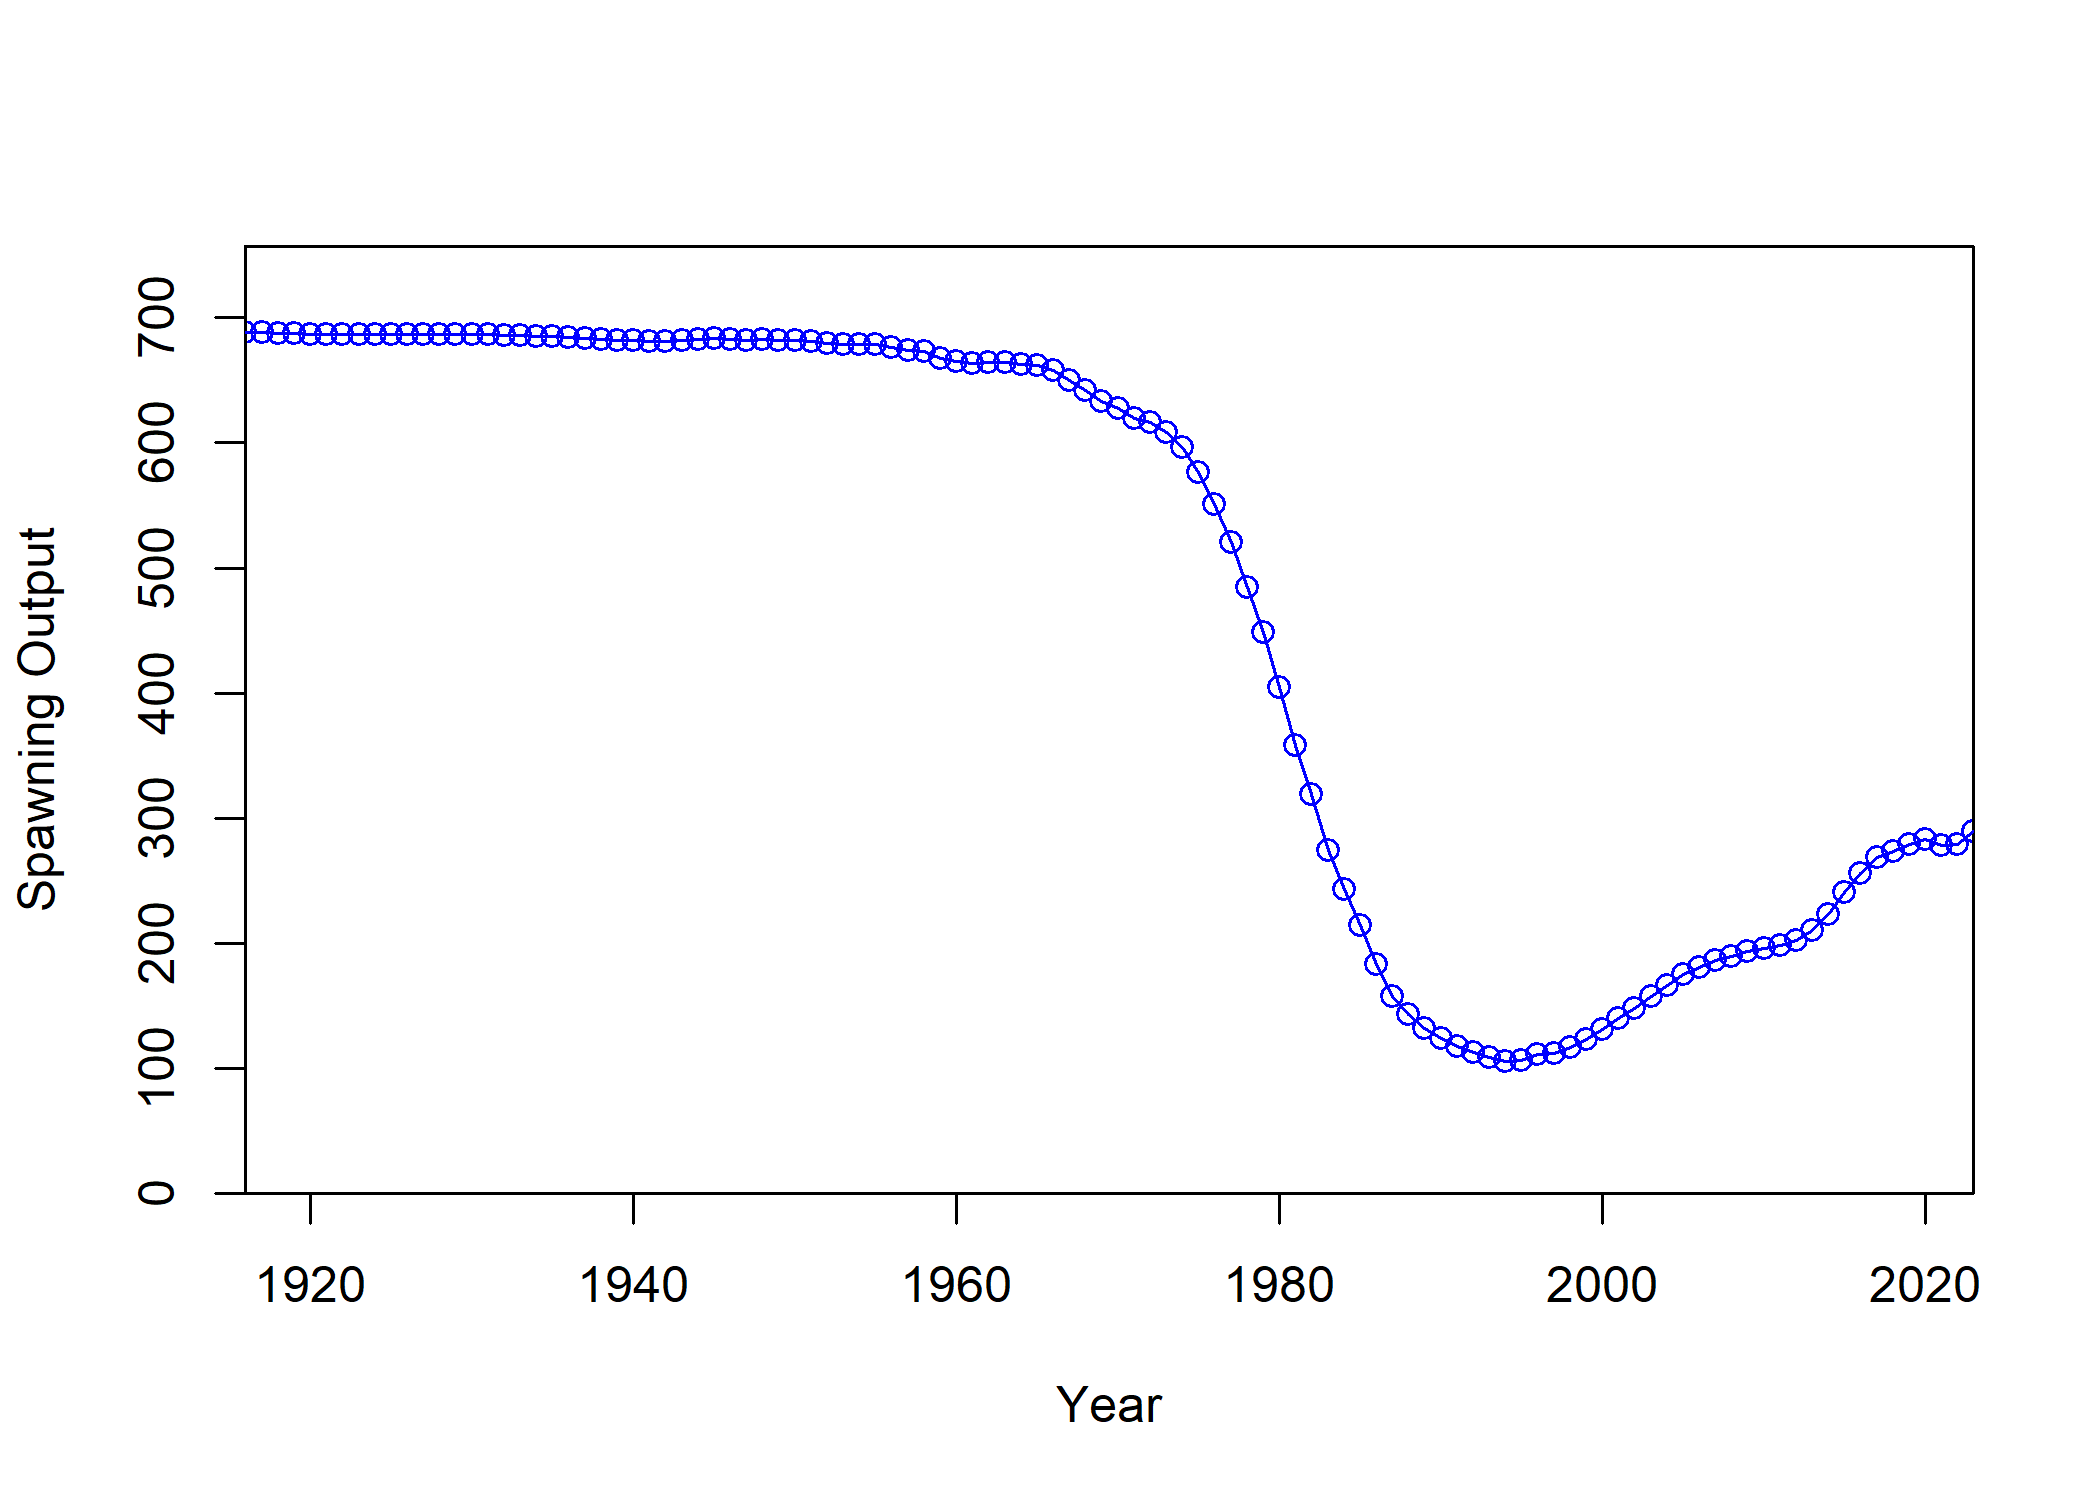
\includegraphics[alt=See Table 23.,width=1\textwidth,height=1\textheight]{C:/Users/melissa.monk/Documents/GitHub/copper_rockfish_2023/documents/shared_figures/spawning_output_combined.png}
}
\caption{Estimated combined time series of spawning output for copper rockfish in California waters.\label{fig:es-sb-all}}
\end{figure}

\begin{figure}
{\centering
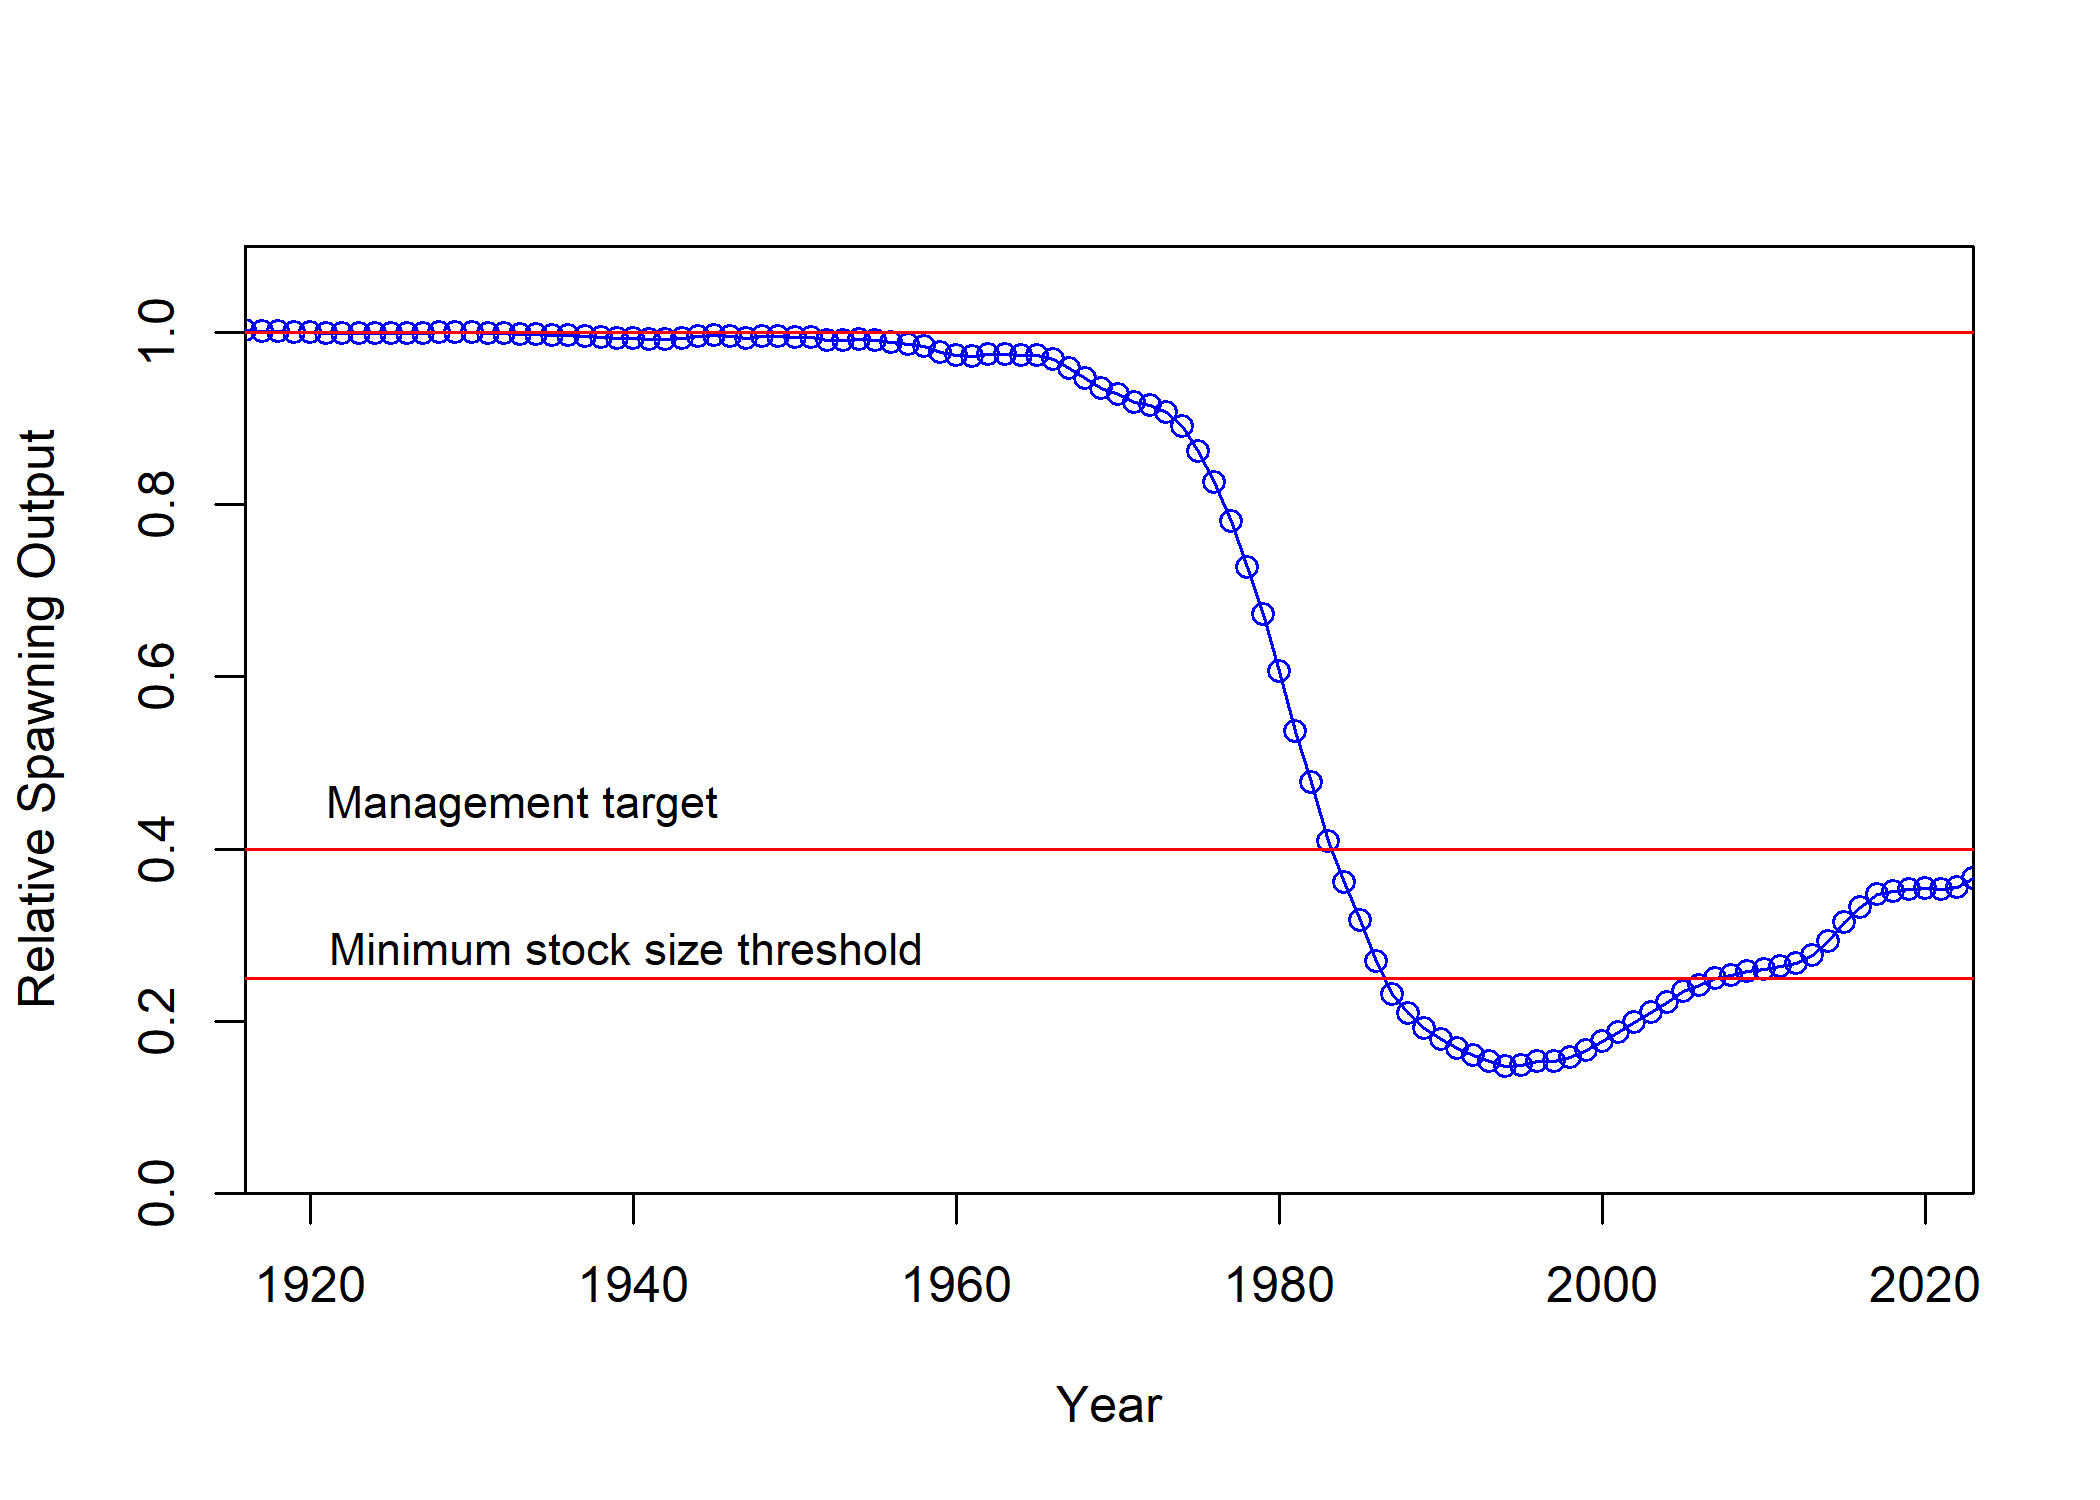
\includegraphics[alt=See Table 23.,width=1\textwidth,height=1\textheight]{C:/Users/melissa.monk/Documents/GitHub/copper_rockfish_2023/documents/shared_figures/depletion_combined.png}
}
\caption{Estimated combined time series of fraction of relative spawning output for copper rockfish in California waters.\label{fig:es-depl-all}}
\end{figure}

\begin{figure}
{\centering
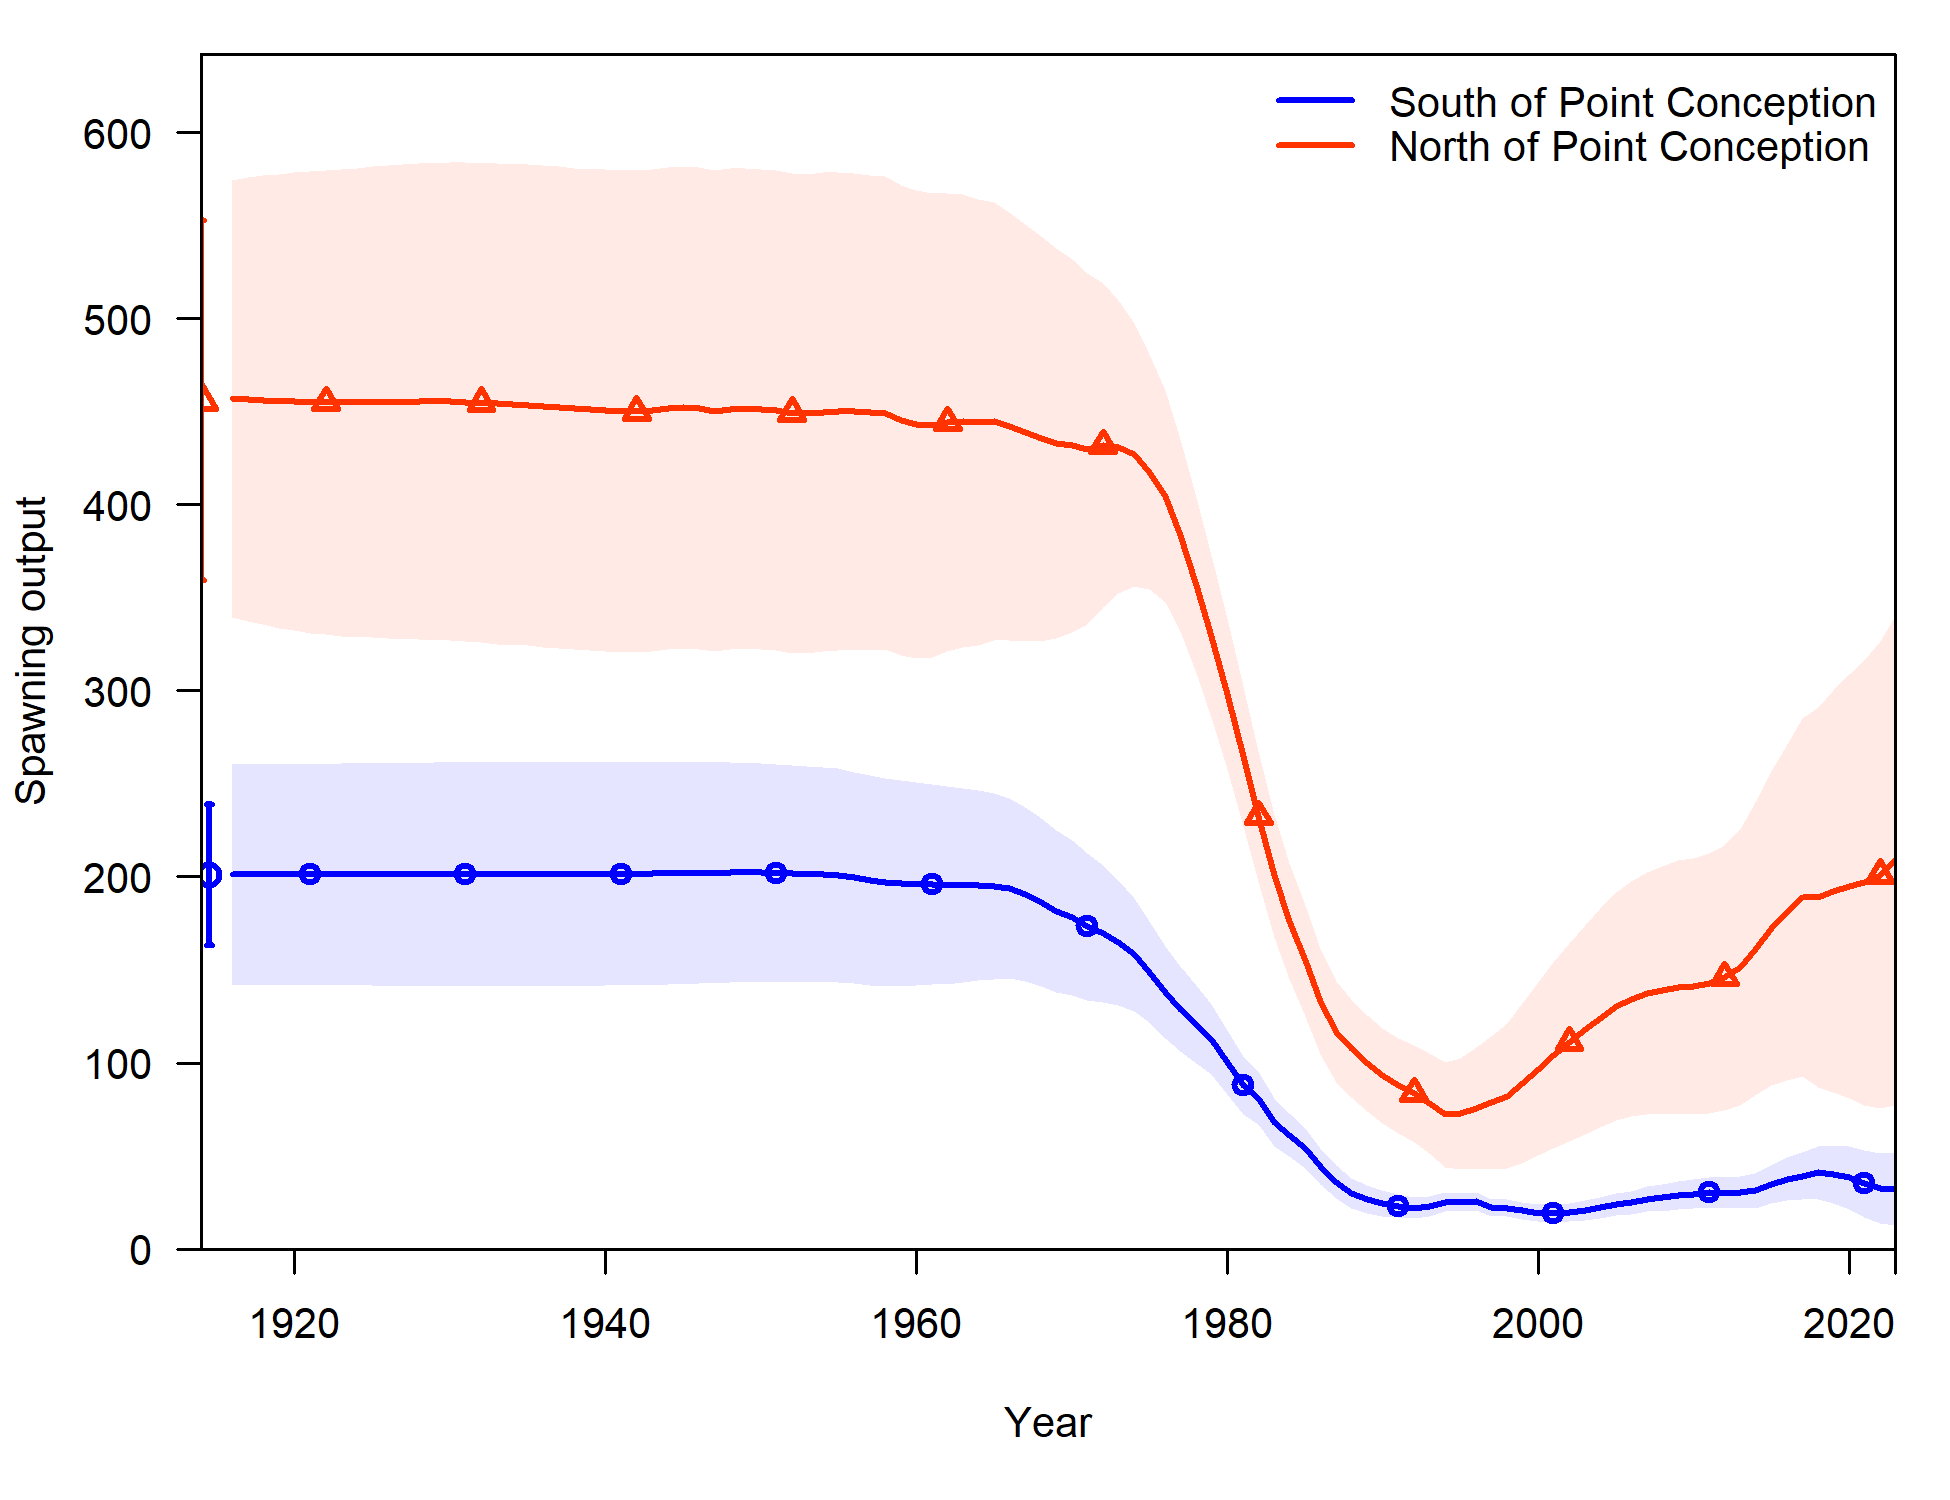
\includegraphics[alt=See Table 22 in this document and Table 15 in the north of Point Conception assessment document.,width=1\textwidth,height=1\textheight]{C:/Users/melissa.monk/Documents/GitHub/copper_rockfish_2023/documents/shared_figures/compare2_spawnbio_uncertainty.png}
}
\caption{Estimated time series of spawning output (circles and line: median; light broken lines: 95 percent intervals) for the model areas south and north of Point Conception.\label{fig:es-sb}}
\end{figure}

\begin{figure}
{\centering
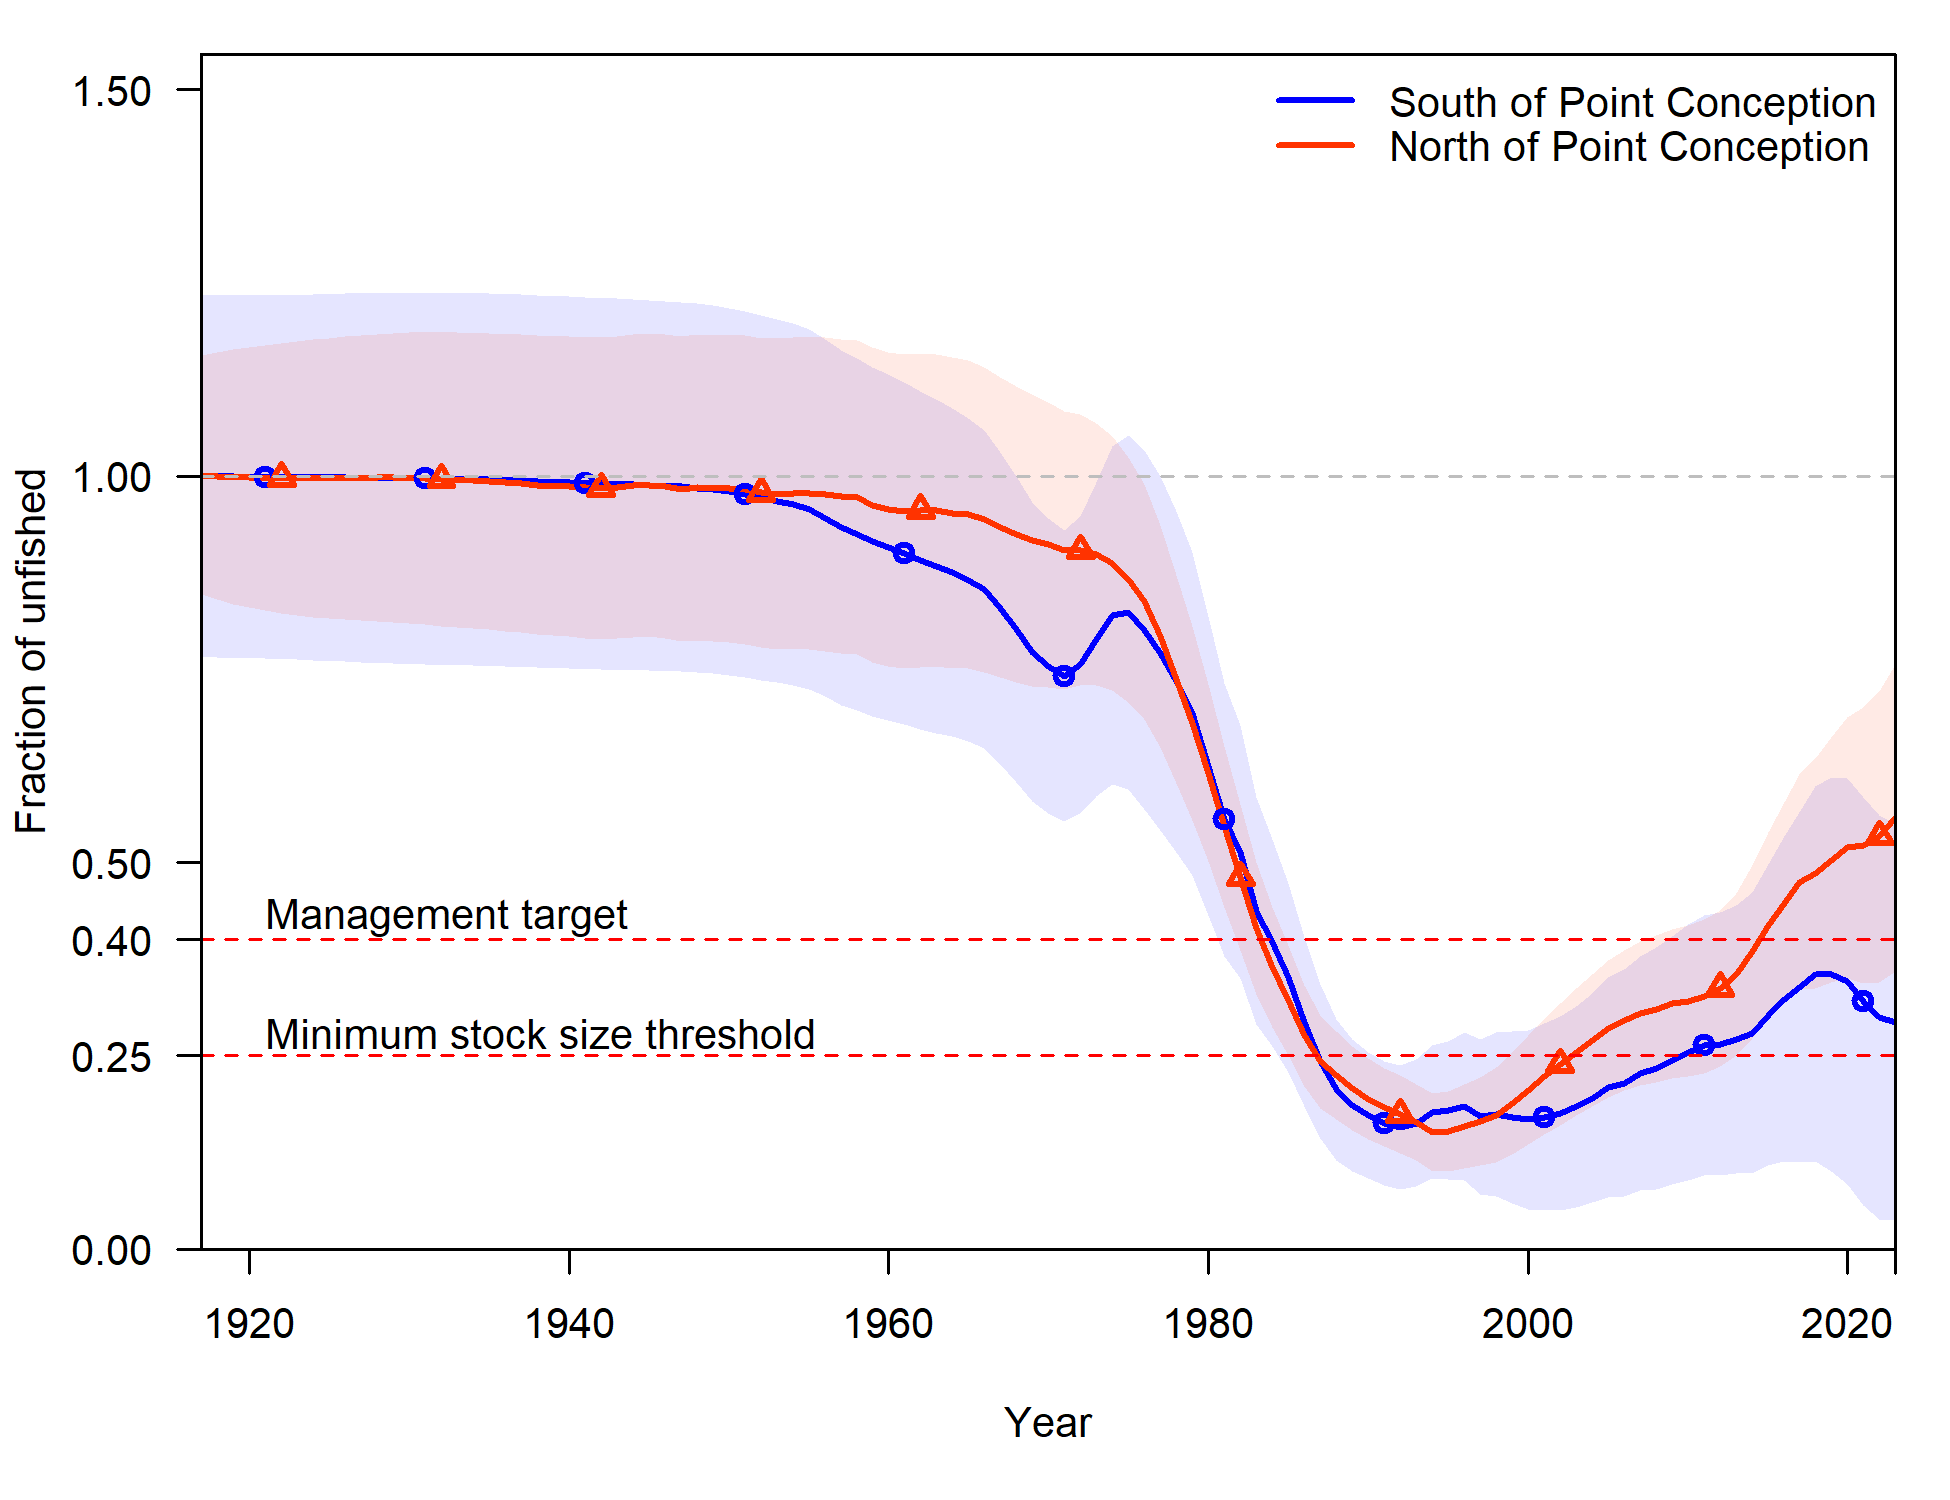
\includegraphics[alt=See Table 22 in this document and Table 15 in the north of Point Conception assessment document.,width=1\textwidth,height=1\textheight]{C:/Users/melissa.monk/Documents/GitHub/copper_rockfish_2023/documents/shared_figures/compare4_Bratio_uncertainty.png}
}
\caption{Estimated time series of fraction of relative spawning output (circles and line: median; light broken lines: 95 percent intervals) for the model areas south and north of Point Conception.\label{fig:es-depl}}
\end{figure}

\pagebreak

\subsection*{Recruitment}\label{recruitment}
\addcontentsline{toc}{subsection}{Recruitment}

Recruitment deviations were estimated from 1965-2020 south of Point Conception and from 1970-2019 north of Point Conception. The estimated magnitude of recruitment deviations and years of strong or weak recruitment varied for each sub-area. The base model south of Point Conception estimated strong recruitment in 2009, 2010, and 2013 with multiple poor recruitment years at the end of the time series (Table \ref{tab:south-recrES} and Figures \ref{fig:es-recruits} and \ref{fig:es-rec-devs}). The sub-area model north of Point Conception estimated the largest recent recruitment deviations in 2007, 2009, and 2017 with series of poor recruitment occurring in the late 1990s and early 2000s (Table \ref{tab:north-recrES} and Figures \ref{fig:es-recruits} and \ref{fig:es-rec-devs}). The magnitude of overall estimated relative recruitment variation, highs and lows, was greater in the sub-area south of Point Conception compared to the sub-area north of Point Conception.

\begingroup\fontsize{10}{12}\selectfont
\begingroup\fontsize{10}{12}\selectfont

\begin{longtable}[t]{r>{\centering\arraybackslash}p{1.57cm}>{\centering\arraybackslash}p{1.57cm}>{\centering\arraybackslash}p{1.57cm}>{\centering\arraybackslash}p{1.57cm}>{\centering\arraybackslash}p{1.57cm}>{\centering\arraybackslash}p{1.57cm}}
\caption{\label{tab:south-recrES}Estimated recent trend in recruitment and recruitment deviations and the 95 percent intervals for the sub-area model south of Point Conception.}\\
\toprule
Year & Recruitment & Lower Interval & Upper Interval & Recruitment Deviations & Lower Interval & Upper Interval\\
\midrule
\endfirsthead
\caption[]{Estimated recent trend in recruitment and recruitment deviations and the 95 percent intervals for the sub-area model south of Point Conception. \textit{(continued)}}\\
\toprule
Year & Recruitment & Lower Interval & Upper Interval & Recruitment Deviations & Lower Interval & Upper Interval\\
\midrule
\endhead

\endfoot
\bottomrule
\endlastfoot
2013 & 613.62 & 381.00 & 988.26 & 1.18 & 0.94 & 1.41\\
2014 & 168.22 & 86.76 & 326.18 & -0.13 & -0.64 & 0.39\\
2015 & 81.26 & 39.81 & 165.88 & -0.88 & -1.45 & -0.30\\
2016 & 114.55 & 59.49 & 220.57 & -0.55 & -1.00 & -0.09\\
2017 & 91.14 & 44.28 & 187.61 & -0.79 & -1.33 & -0.25\\
2018 & 91.39 & 42.11 & 198.33 & -0.80 & -1.40 & -0.19\\
2019 & 119.56 & 51.10 & 279.76 & -0.53 & -1.24 & 0.18\\
2020 & 119.75 & 43.77 & 327.64 & -0.60 & -1.54 & 0.34\\
2021 & 231.44 & 144.36 & 371.04 & 0.00 & 0.00 & 0.00\\
2022 & 227.42 & 138.88 & 372.42 & 0.00 & 0.00 & 0.00\\
2023 & 226.18 & 137.68 & 371.57 & 0.00 & 0.00 & 0.00\\*
\end{longtable}
\endgroup{}
\endgroup{}


\newpage

\begingroup\fontsize{10}{12}\selectfont
\begingroup\fontsize{10}{12}\selectfont

\begin{longtable}[t]{r>{\centering\arraybackslash}p{1.57cm}>{\centering\arraybackslash}p{1.57cm}>{\centering\arraybackslash}p{1.57cm}>{\centering\arraybackslash}p{1.57cm}>{\centering\arraybackslash}p{1.57cm}>{\centering\arraybackslash}p{1.57cm}}
\caption{\label{tab:north-recrES}Estimated recent trend in recruitment and recruitment deviations and the 95 percent intervals for the sub-area model north of Point Conception.}\\
\toprule
Year & Recruitment & Lower Interval & Upper Interval & Recruitment Deviations & Lower Interval & Upper Interval\\
\midrule
\endfirsthead
\caption[]{Estimated recent trend in recruitment and recruitment deviations and the 95 percent intervals for the sub-area model north of Point Conception. \textit{(continued)}}\\
\toprule
Year & Recruitment & Lower Interval & Upper Interval & Recruitment Deviations & Lower Interval & Upper Interval\\
\midrule
\endhead

\endfoot
\bottomrule
\endlastfoot
2013 & 556.60 & 282.67 & 1095.99 & 0.23 & -0.38 & 0.84\\
2014 & 466.50 & 233.22 & 933.12 & 0.04 & -0.59 & 0.67\\
2015 & 590.78 & 316.19 & 1103.84 & 0.26 & -0.27 & 0.79\\
2016 & 285.96 & 134.46 & 608.15 & -0.47 & -1.18 & 0.24\\
2017 & 869.76 & 474.53 & 1594.18 & 0.63 & 0.13 & 1.12\\
2018 & 618.32 & 318.82 & 1199.18 & 0.25 & -0.34 & 0.84\\
2019 & 345.34 & 159.74 & 746.57 & -0.37 & -1.11 & 0.37\\
2020 & 502.19 & 394.01 & 640.08 & 0.00 & 0.00 & 0.00\\
2021 & 503.74 & 394.44 & 643.32 & 0.00 & 0.00 & 0.00\\
2022 & 505.86 & 395.70 & 646.68 & 0.00 & 0.00 & 0.00\\
2023 & 509.39 & 398.85 & 650.56 & 0.00 & 0.00 & 0.00\\*
\end{longtable}
\endgroup{}
\endgroup{}


\begin{figure}
{\centering
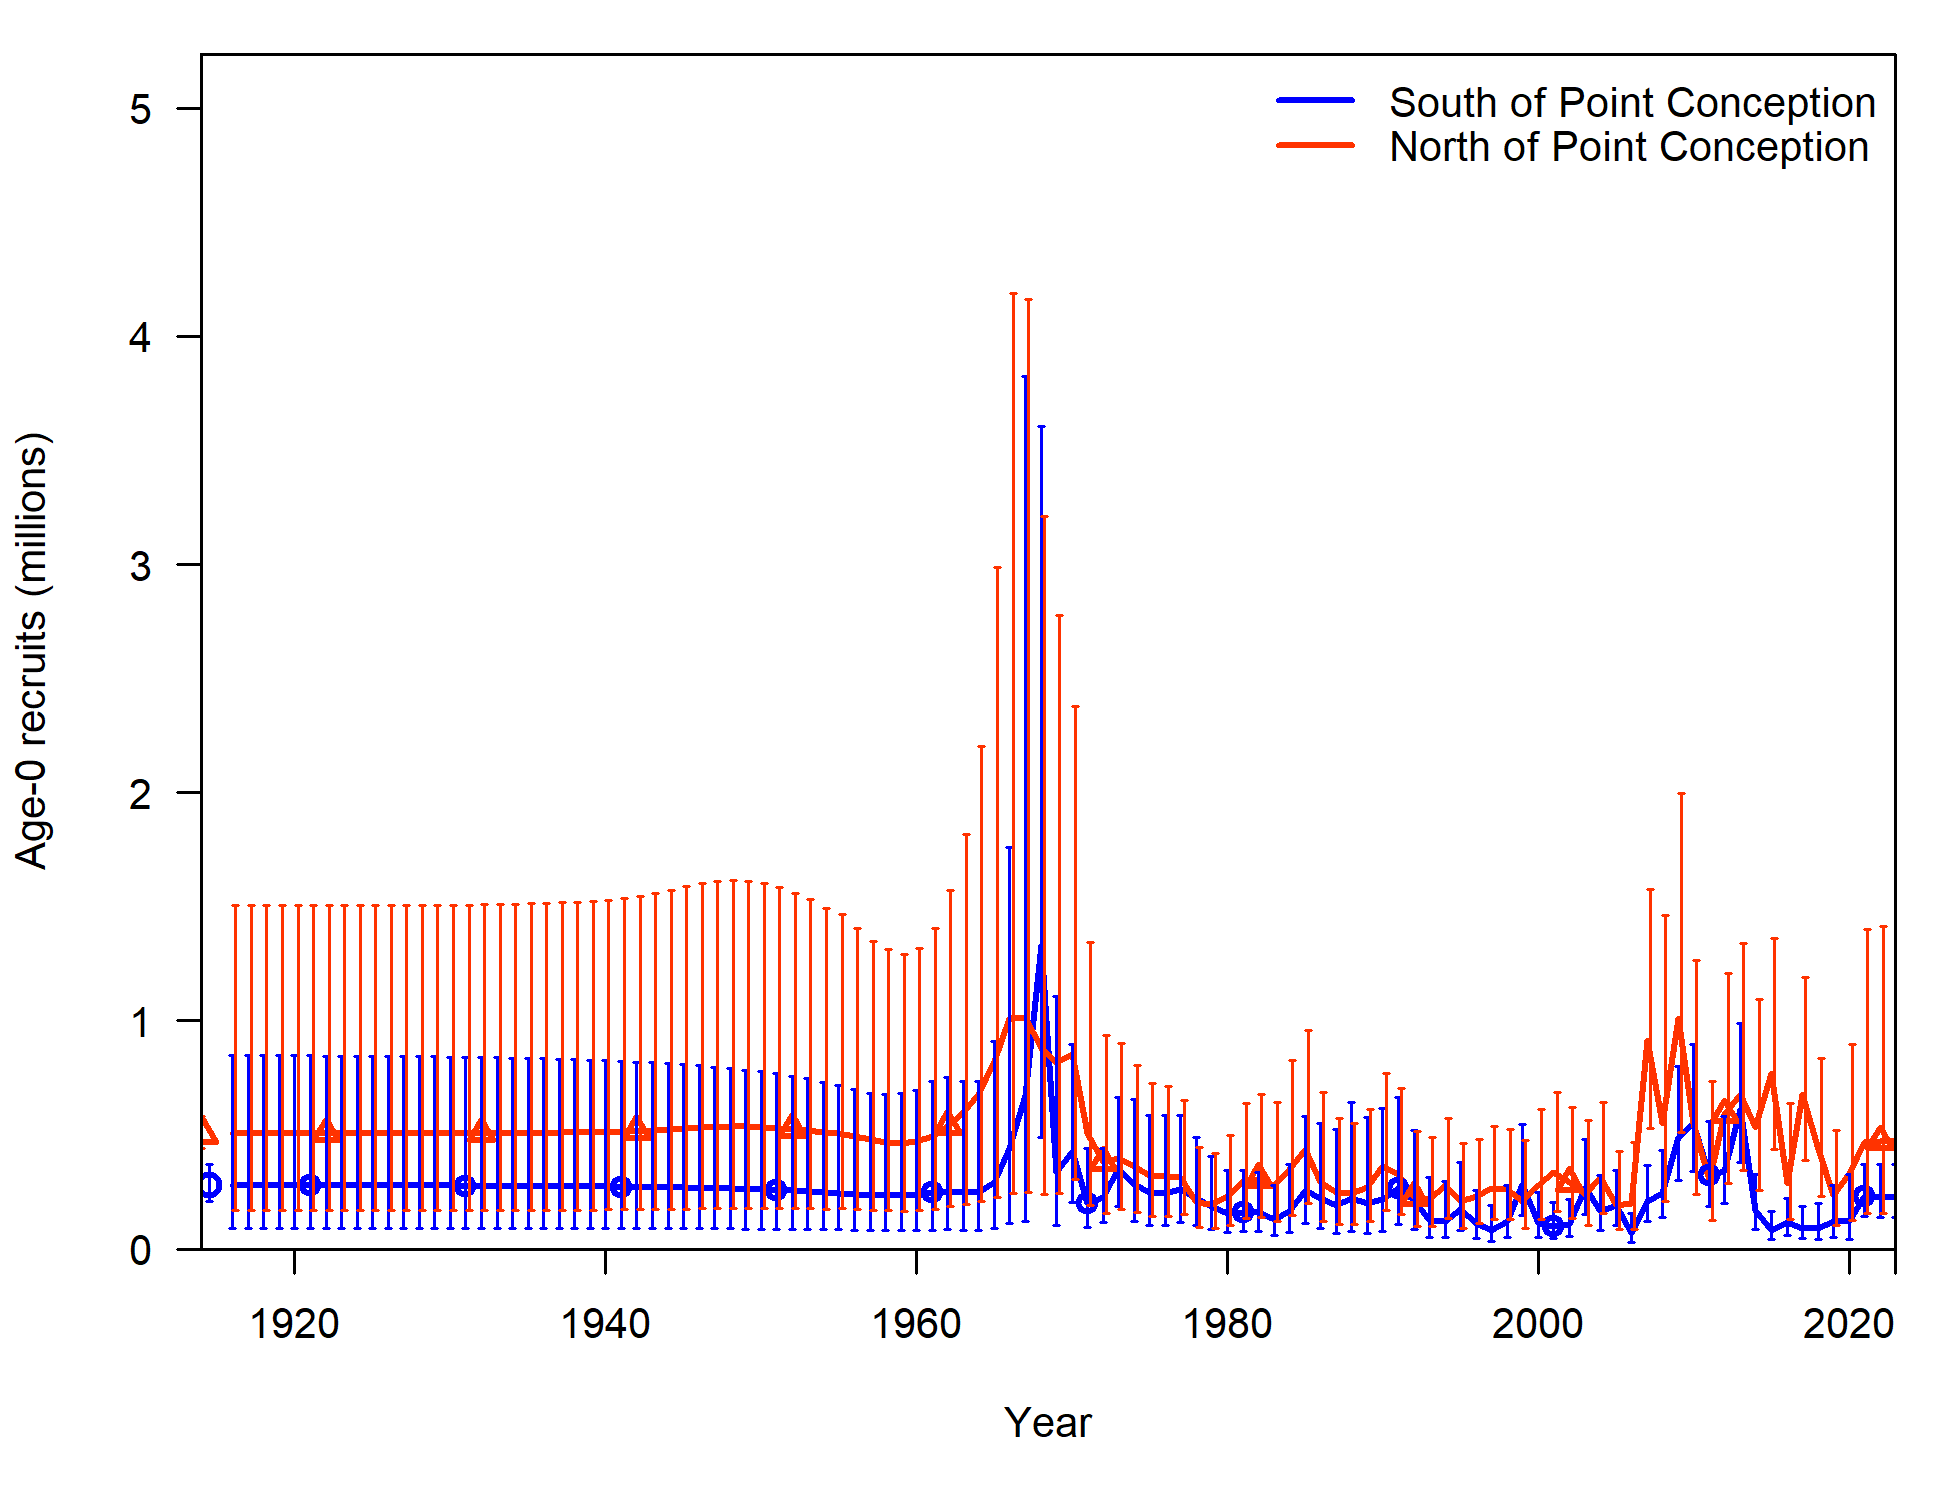
\includegraphics[alt=See Table 22 in this document and Table 15 in the north of Point Conception assessment document.,width=1\textwidth,height=1\textheight]{C:/Users/melissa.monk/Documents/GitHub/copper_rockfish_2023/documents/shared_figures/compare10_recruits_uncertainty.png}
}
\caption{Estimated time series of age-0 recruits (1000s) for the model areas south and north of Point Conception with 95 percent intervals.\label{fig:es-recruits}}
\end{figure}

\begin{figure}
{\centering
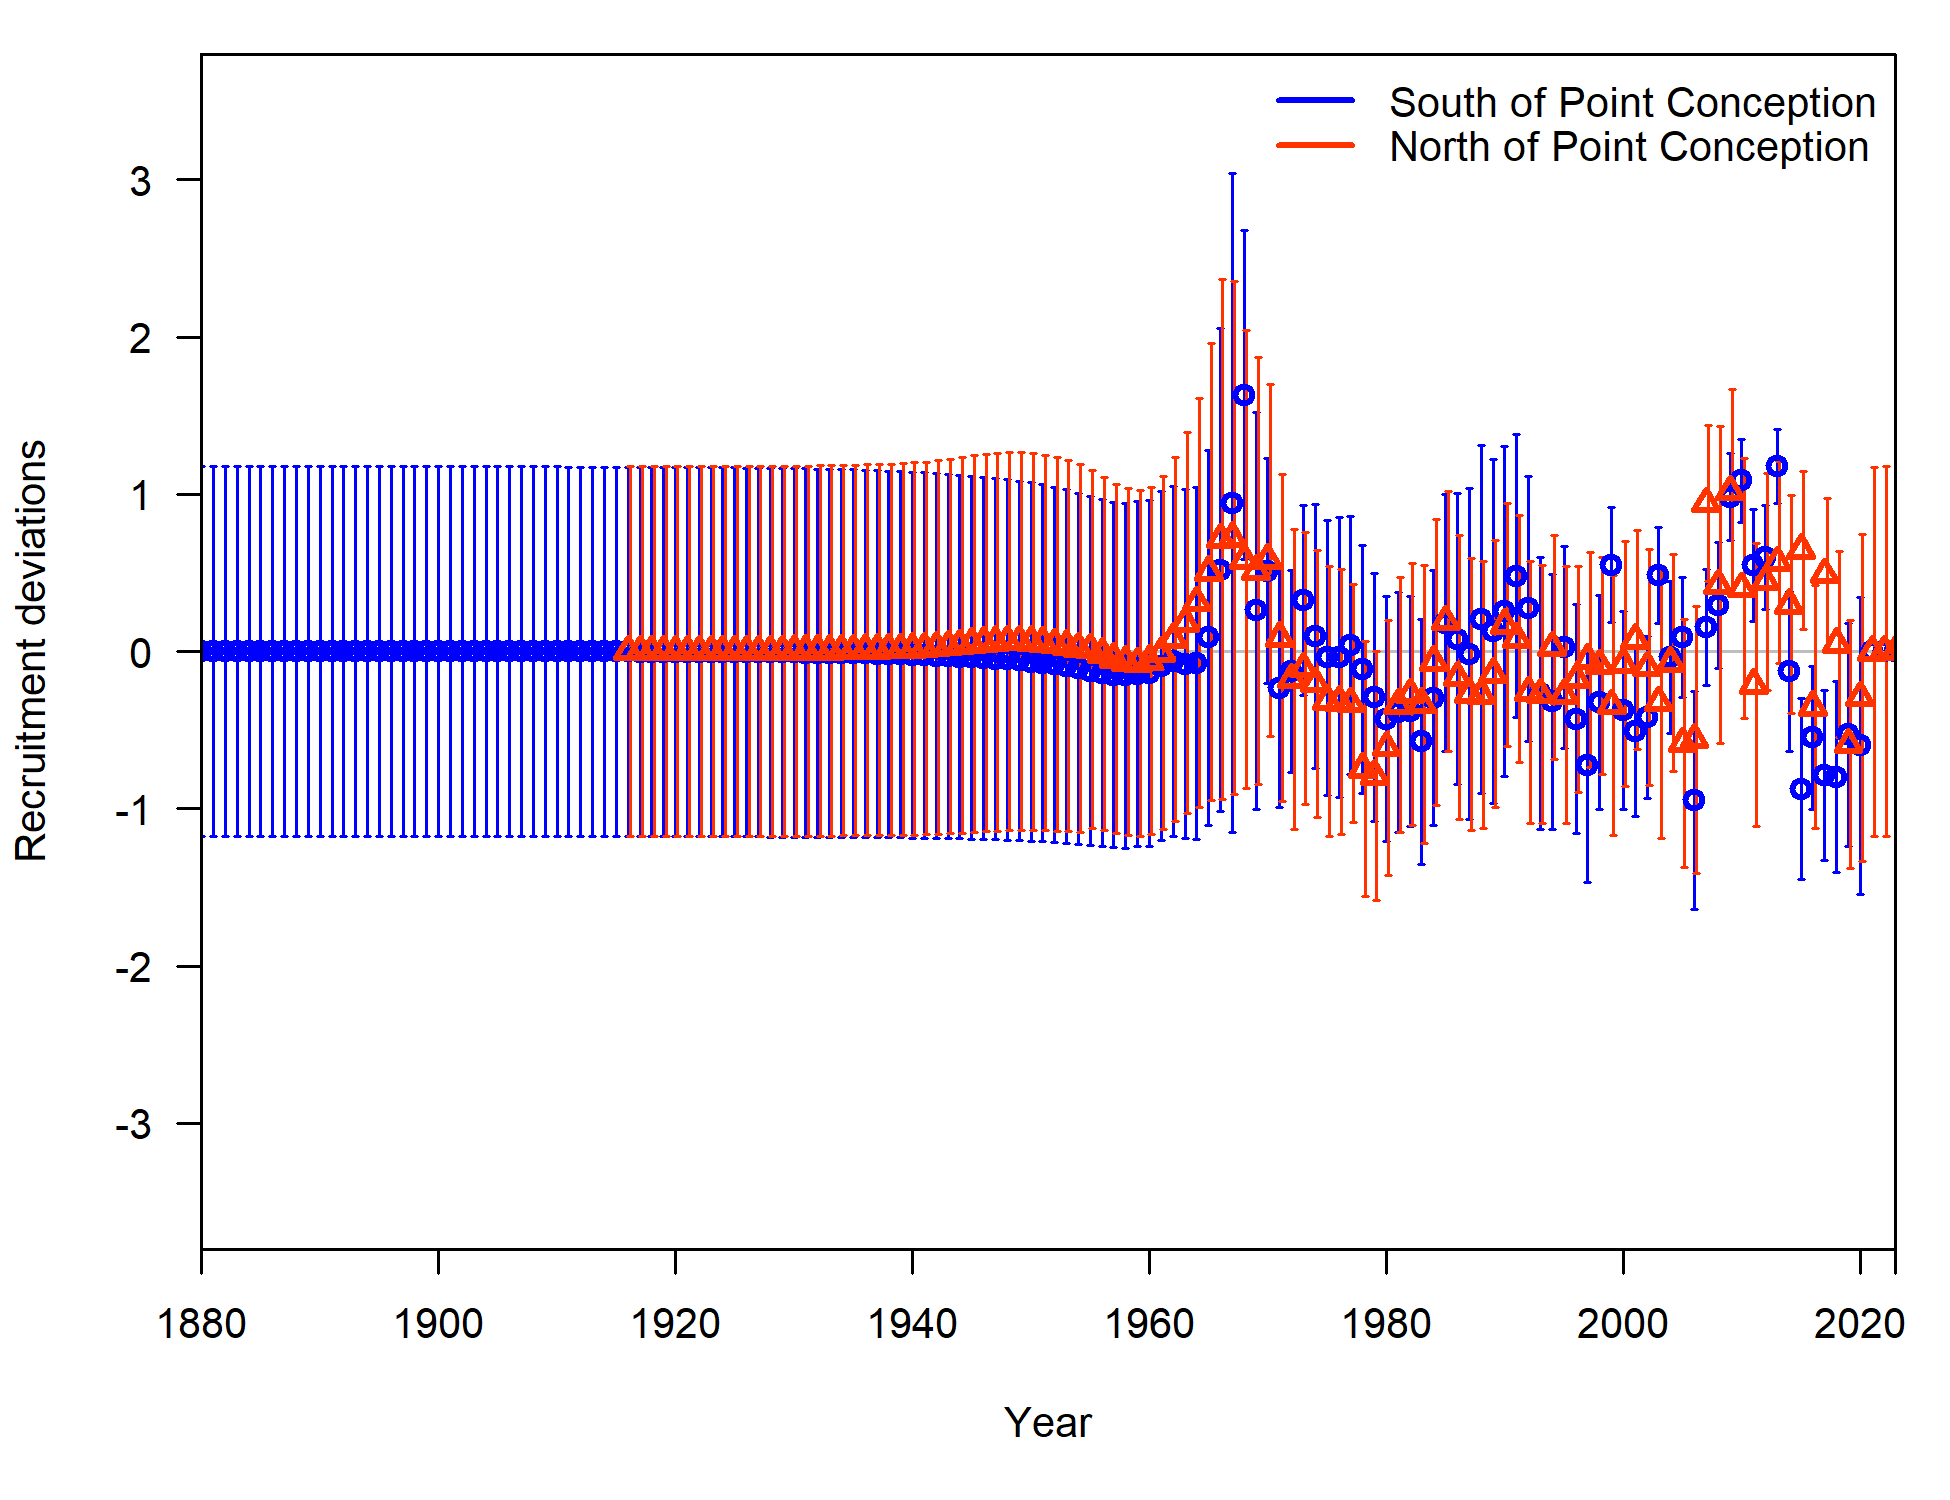
\includegraphics[alt=See Table vi and vii.,width=1\textwidth,height=1\textheight]{C:/Users/melissa.monk/Documents/GitHub/copper_rockfish_2023/documents/shared_figures/compare12_recdevs_uncertainty.png}
}
\caption{Estimated time series of recruitment deviations for the model areas south and north of Point Conception.\label{fig:es-rec-devs}}
\end{figure}

\clearpage

\subsection*{Exploitation status}\label{exploitation-status}
\addcontentsline{toc}{subsection}{Exploitation status}

Trends in fishing intensity (1 - SPR) for both sub-areas dramatically increased in the 1970s, exceeded the management target \(\text{SPR}_{50\%}\), and remained high until at least the late 1990s (Figure \ref{fig:es-1-spr}). The fishing intensity south of Point Conception declined in the early 2000s but remained above the target for the rest of the time series except for 2006 (Table \ref{tab:south-exploitES}). The fishing intensity sharply decreased around 2000 north of Point Conception with fishing intensity remaining below the management target since, excluding a recent spike in 2017 (Table \ref{tab:north-exploitES}).

As a percentage of biomass (ages 3+), harvest rates south of Point Conception between 2013-2021 ranged between 0.13-0.19, with harvest rates declining in 2022 to 0.06 based on inseason management actions by California Department of Fish and Wildlife (CDFW) that reduced the sub-bag limit for copper rockfish to one fish across the state (Table \ref{tab:south-exploitES}). The harvest rates in the sub-area north of Point Conception since 2013 have ranged between 0.01-0.07 (Table \ref{tab:north-exploitES}).

\begingroup\fontsize{10}{12}\selectfont
\begingroup\fontsize{10}{12}\selectfont

\begin{longtable}[t]{r>{\centering\arraybackslash}p{1.57cm}>{\centering\arraybackslash}p{1.57cm}>{\centering\arraybackslash}p{1.57cm}>{\centering\arraybackslash}p{1.57cm}>{\centering\arraybackslash}p{1.57cm}>{\centering\arraybackslash}p{1.57cm}}
\caption{\label{tab:south-exploitES}Estimated recent trend in the 1-SPR where SPR is the spawning potential ratio the exploitation rate, and the 95 percent intervals for the sub-area model south of Point Conception.}\\
\toprule
Year & 1-SPR & Lower Interval & Upper Interval & Exploitation Rate & Lower Interval & Upper Interval\\
\midrule
\endfirsthead
\caption[]{Estimated recent trend in the 1-SPR where SPR is the spawning potential ratio the exploitation rate, and the 95 percent intervals for the sub-area model south of Point Conception. \textit{(continued)}}\\
\toprule
Year & 1-SPR & Lower Interval & Upper Interval & Exploitation Rate & Lower Interval & Upper Interval\\
\midrule
\endhead

\endfoot
\bottomrule
\endlastfoot
2013 & 0.71 & 0.52 & 0.90 & 0.11 & 0.05 & 0.17\\
2014 & 0.59 & 0.39 & 0.79 & 0.08 & 0.04 & 0.13\\
2015 & 0.66 & 0.46 & 0.86 & 0.10 & 0.05 & 0.16\\
2016 & 0.71 & 0.51 & 0.90 & 0.12 & 0.05 & 0.18\\
2017 & 0.67 & 0.46 & 0.88 & 0.10 & 0.04 & 0.16\\
2018 & 0.75 & 0.55 & 0.95 & 0.12 & 0.05 & 0.20\\
2019 & 0.72 & 0.50 & 0.94 & 0.11 & 0.03 & 0.18\\
2020 & 0.80 & 0.59 & 1.01 & 0.12 & 0.03 & 0.21\\
2021 & 0.72 & 0.47 & 0.98 & 0.09 & 0.02 & 0.17\\
2022 & 0.40 & 0.15 & 0.64 & 0.03 & 0.01 & 0.06\\*
\end{longtable}
\endgroup{}
\endgroup{}


\newpage

\begingroup\fontsize{10}{12}\selectfont
\begingroup\fontsize{10}{12}\selectfont

\begin{longtable}[t]{r>{\centering\arraybackslash}p{1.57cm}>{\centering\arraybackslash}p{1.57cm}>{\centering\arraybackslash}p{1.57cm}>{\centering\arraybackslash}p{1.57cm}>{\centering\arraybackslash}p{1.57cm}>{\centering\arraybackslash}p{1.57cm}}
\caption{\label{tab:north-exploitES}Estimated recent trend in the 1-SPR where SPR is the spawning potential ratio the exploitation rate, and the 95 percent intervals for the sub-area model north of Point Conception.}\\
\toprule
Year & 1-SPR & Lower Interval & Upper Interval & Exploitation Rate & Lower Interval & Upper Interval\\
\midrule
\endfirsthead
\caption[]{Estimated recent trend in the 1-SPR where SPR is the spawning potential ratio the exploitation rate, and the 95 percent intervals for the sub-area model north of Point Conception. \textit{(continued)}}\\
\toprule
Year & 1-SPR & Lower Interval & Upper Interval & Exploitation Rate & Lower Interval & Upper Interval\\
\midrule
\endhead

\endfoot
\bottomrule
\endlastfoot
2013 & 0.16 & 0.10 & 0.22 & 0.01 & 0.01 & 0.02\\
2014 & 0.20 & 0.13 & 0.27 & 0.02 & 0.01 & 0.02\\
2015 & 0.31 & 0.21 & 0.41 & 0.03 & 0.02 & 0.04\\
2016 & 0.31 & 0.20 & 0.41 & 0.03 & 0.02 & 0.04\\
2017 & 0.50 & 0.37 & 0.63 & 0.05 & 0.03 & 0.08\\
2018 & 0.41 & 0.28 & 0.53 & 0.04 & 0.02 & 0.06\\
2019 & 0.40 & 0.27 & 0.53 & 0.04 & 0.02 & 0.06\\
2020 & 0.53 & 0.38 & 0.67 & 0.06 & 0.03 & 0.08\\
2021 & 0.41 & 0.27 & 0.55 & 0.04 & 0.02 & 0.06\\
2022 & 0.21 & 0.12 & 0.30 & 0.02 & 0.01 & 0.03\\*
\end{longtable}
\endgroup{}
\endgroup{}


\begin{figure}
{\centering
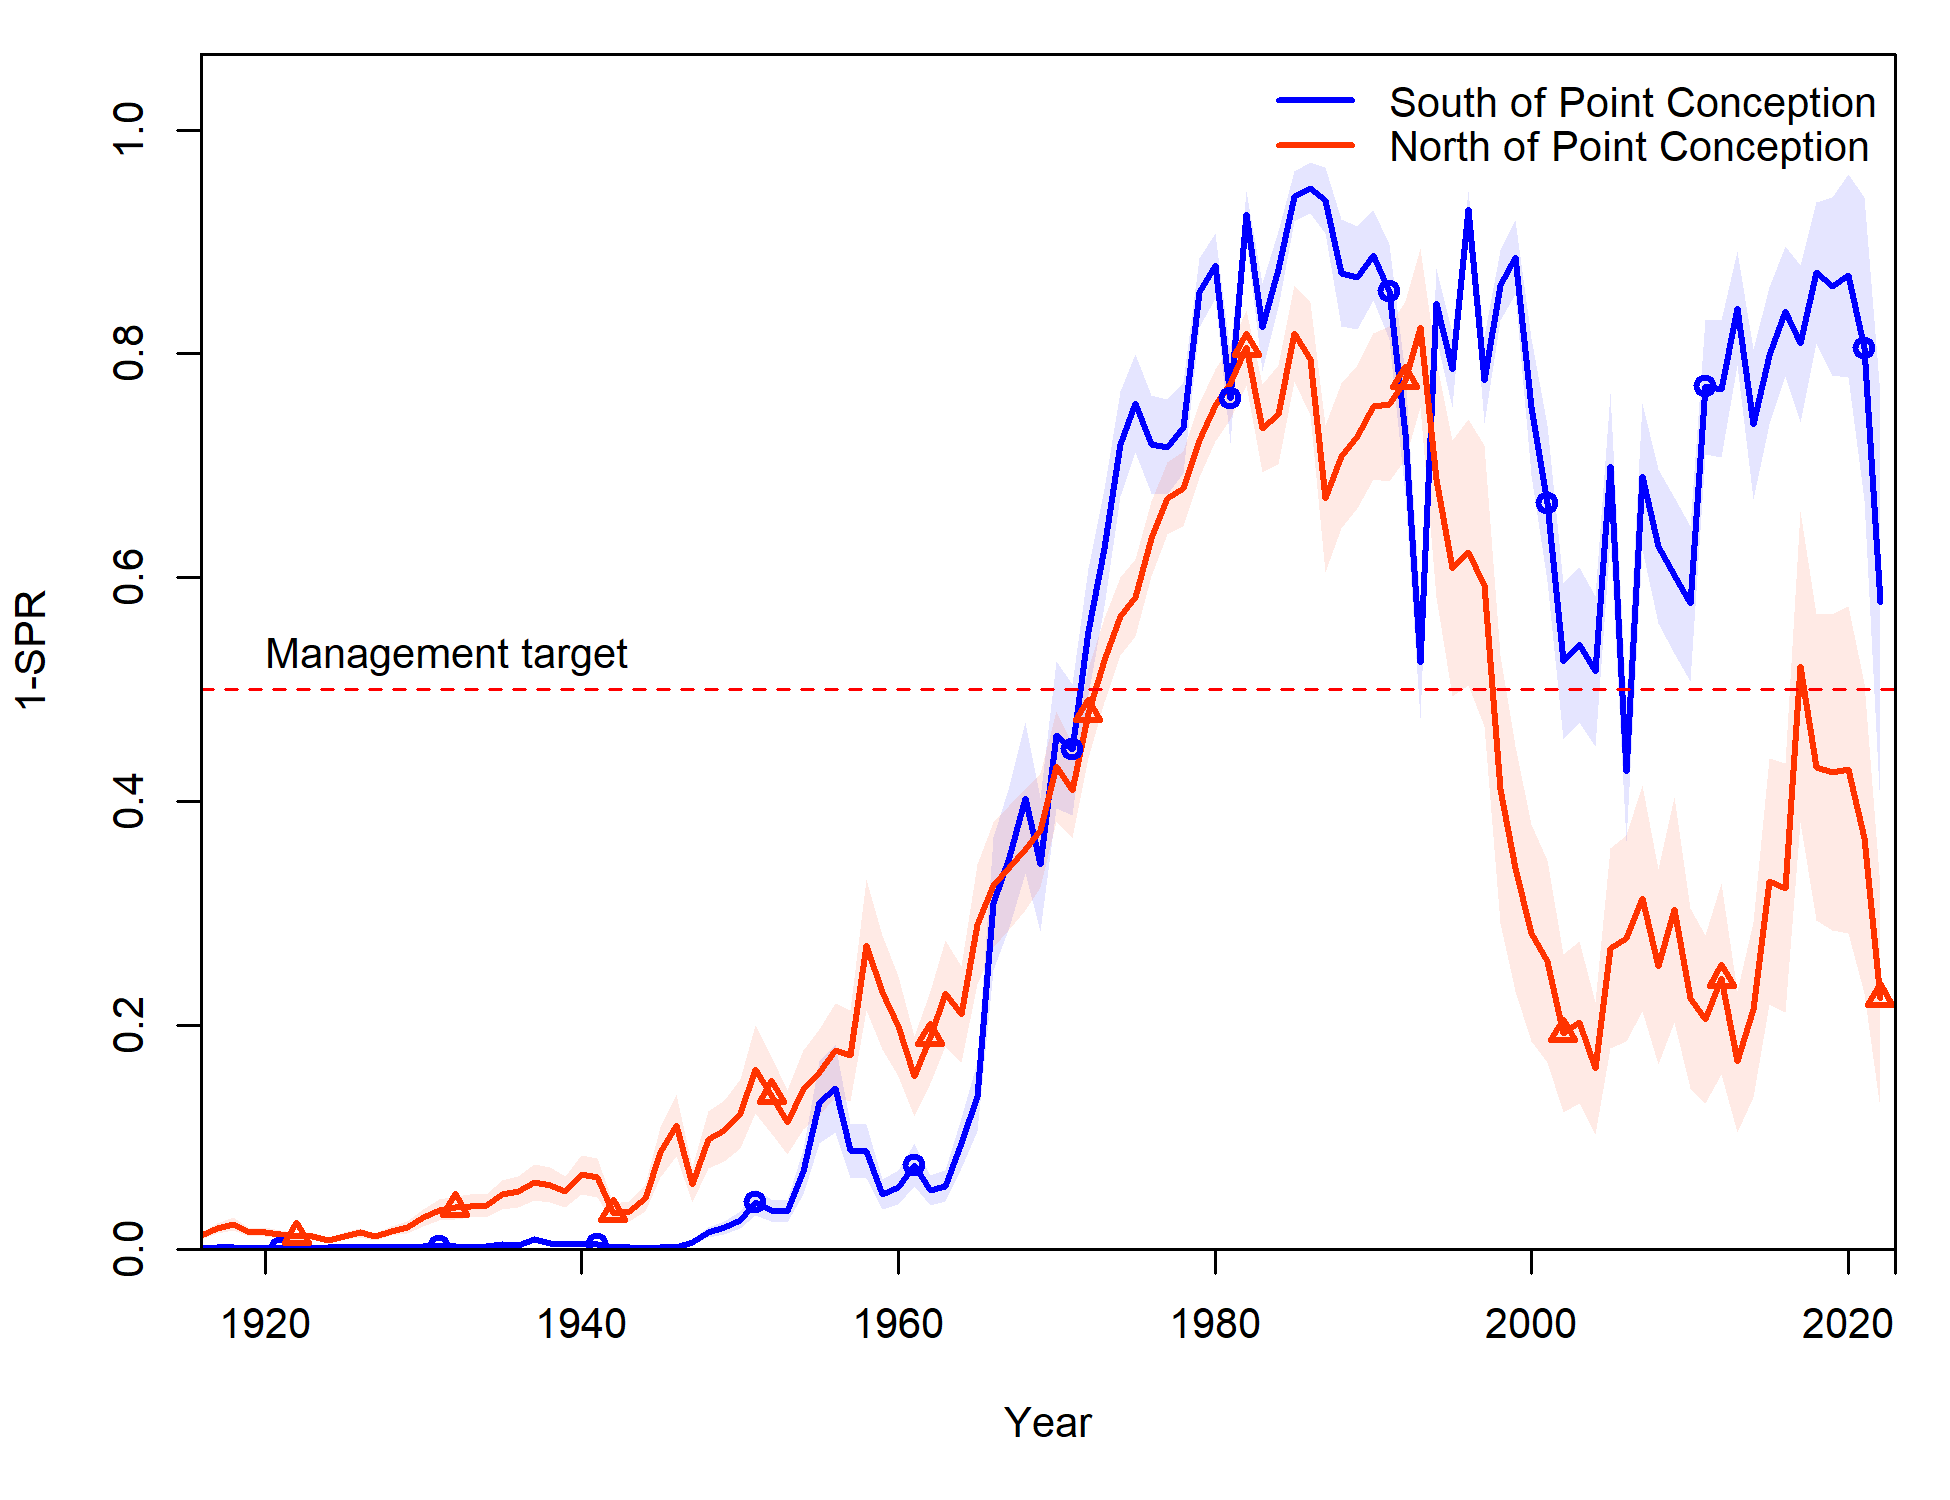
\includegraphics[alt=See Table 22 in this document and Table 15 in the north of Point Conception assessment document.,width=1\textwidth,height=1\textheight]{C:/Users/melissa.monk/Documents/GitHub/copper_rockfish_2023/documents/shared_figures/compare6_SPRratio_uncertainty.png}
}
\caption{Estimated 1 - relative spawning ratio (SPR) by year for the model areas south and north of Point Conception. The management target is plotted as a red horizontal line and values above this reflect harvest in excess of the proxy harvest rate.\label{fig:es-1-spr}}
\end{figure}

\pagebreak

\subsection*{Ecosystem considerations}\label{ecosystem-considerations}
\addcontentsline{toc}{subsection}{Ecosystem considerations}

This stock assessment does not explicitly incorporate trophic interactions, habitat factors (other than as they inform relative abundance indices) or environmental factors into the assessment model, but a brief description of likely or potential ecosystem considerations is provided below.

As with most other rockfish and groundfish in the California Current, recruitment or cohort (year-class) strength appears to be highly variable for copper rockfish, with only a modest apparent relationship to estimated levels of spawning output. Oceanographic and ecosystem factors are widely recognized to be key drivers of recruitment variability for most species of groundfish, as well as most elements of California Current food webs. Empirical estimates of recruitment from pelagic juvenile rockfish surveys have been used to inform incoming year class strength for some of these stocks, however copper rockfish are infrequently encountered in these surveys. Between 1998 and 2013 the California Cooperative Oceanic Fisheries Investigation (CalCOFI) survey had 34 positive observations of copper rockfish out of over 500 bongo net tows.

\subsection*{Reference points}\label{reference-points}
\addcontentsline{toc}{subsection}{Reference points}

Reference points were calculated using the estimated selectivities and catch distribution among fleets in the final year of each sub-area model, 2022. Reference points are presented in Tables \ref{tab:south-referenceES} and \ref{tab:north-referenceES} for each sub-model area and are informational only. Copper rockfish off the California coast are managed as a single stock by the Pacific Fishery Management Council. Combined reference point quantities for the California stock are shown in Table \ref{tab:ref-point-all-es}.

Sustainable total yield (landings plus discards) across California is estimated to 164.24 mt when using an \(\text{SPR}_{50\%}\) reference harvest rate. The spawning output equivalent to 40 percent of the unfished level (\(\text{SO}_{40\%}\)) was 262.8 billions of eggs.

The 2022 combined California spawning output relative to unfished equilibrium spawning biomass is at 37 percent of unfished, below the management target of 40 percent (Table \ref{tab:es-ca-status}). The fishing intensity, \(1-\text{SPR}\), for each model area varied where the portion of the stock north of Point Conception has been below that target in recent years (Figures \ref{fig:es-1-spr} and \ref{fig:es-phase}). In contrast, the fishing intensity south of Point Conception has been estimated to be above the target in recent years.

Tables \ref{tab:south-referenceES} and \ref{tab:north-referenceES} show the full suite of estimated reference points for each sub-area model and Figures \ref{fig:south-es-yield} and \ref{fig:north-es-yield} show the equilibrium yield curves and net production based on a steepness value fixed at 0.72.

\newpage

\begingroup\fontsize{10}{12}\selectfont
\begingroup\fontsize{10}{12}\selectfont

\begin{longtable}[t]{r>{\centering\arraybackslash}p{2cm}>{\centering\arraybackslash}p{2cm}>{\centering\arraybackslash}p{2cm}}
\caption{\label{tab:south-referenceES}Summary of reference points and management quantities, including estimates of the 95 percent intervals for the sub-area model south of Point Conception.}\\
\toprule
 & Estimate & Lower Interval & Upper Interval\\
\midrule
\endfirsthead
\caption[]{Summary of reference points and management quantities, including estimates of the 95 percent intervals for the sub-area model south of Point Conception. \textit{(continued)}}\\
\toprule
 & Estimate & Lower Interval & Upper Interval\\
\midrule
\endhead

\endfoot
\bottomrule
\endlastfoot
Unfished Spawning Output & 201.06 & 163.43 & 238.70\\
Unfished Age 3+ Biomass (mt) & 1999.51 & 1624.90 & 2374.12\\
Unfished Recruitment (R0) & 241.18 & 196.04 & 286.32\\
Spawning Output (2023) & 32.06 & 12.70 & 51.42\\
Fraction Unfished (2023) & 0.16 & 0.06 & 0.25\\
Reference Points Based SB40\% &  &  & \\
Proxy Spawning Output SB40\% & 80.43 & 65.37 & 95.48\\
SPR Resulting in SB40\% & 0.46 & 0.46 & 0.46\\
Exploitation Rate Resulting in SB40\% & 0.06 & 0.05 & 0.06\\
Yield with SPR Based On SB40\% (mt) & 49.99 & 40.74 & 59.25\\
Reference Points Based on SPR Proxy for MSY &  &  & \\
Proxy Spawning Output (SPR50) & 89.71 & 72.92 & 106.50\\
SPR50 & 0.50 & - & -\\
Exploitation Rate Corresponding to SPR50 & 0.05 & 0.05 & 0.05\\
Yield with SPR50 at SB SPR (mt) & 47.78 & 38.93 & 56.62\\
Reference Points Based on Estimated MSY Values &  &  & \\
Spawning Output at MSY (SB MSY) & 55.51 & 45.15 & 65.87\\
SPR MSY & 0.35 & 0.34 & 0.35\\
Exploitation Rate Corresponding to SPR MSY & 0.08 & 0.08 & 0.08\\
MSY (mt) & 52.94 & 43.14 & 62.74\\*
\end{longtable}
\endgroup{}
\endgroup{}


\newpage

\begingroup\fontsize{10}{12}\selectfont
\begingroup\fontsize{10}{12}\selectfont

\begin{longtable}[t]{r>{\centering\arraybackslash}p{2cm}>{\centering\arraybackslash}p{2cm}>{\centering\arraybackslash}p{2cm}}
\caption{\label{tab:north-referenceES}Summary of reference points and management quantities, including estimates of the 95 percent intervals for the sub-area model north of Point Conception.}\\
\toprule
 & Estimate & Lower Interval & Upper Interval\\
\midrule
\endfirsthead
\caption[]{Summary of reference points and management quantities, including estimates of the 95 percent intervals for the sub-area model north of Point Conception. \textit{(continued)}}\\
\toprule
 & Estimate & Lower Interval & Upper Interval\\
\midrule
\endhead

\endfoot
\bottomrule
\endlastfoot
Unfished Spawning Output & 486.15 & 387.43 & 584.87\\
Unfished Age 3+ Biomass (mt) & 4719.91 & 3777.92 & 5661.90\\
Unfished Recruitment (R0) & 567.77 & 452.48 & 683.06\\
Spawning Output (2023) & 262.10 & 124.28 & 399.92\\
Fraction Unfished (2023) & 0.54 & 0.32 & 0.76\\
Reference Points Based SB40\% &  &  & \\
Proxy Spawning Output SB40\% & 194.46 & 154.97 & 233.95\\
SPR Resulting in SB40\% & 0.46 & 0.46 & 0.46\\
Exploitation Rate Resulting in SB40\% & 0.06 & 0.06 & 0.06\\
Yield with SPR Based On SB40\% (mt) & 129.86 & 104.05 & 155.67\\
Reference Points Based on SPR Proxy for MSY &  &  & \\
Proxy Spawning Output (SPR50) & 216.90 & 172.85 & 260.94\\
SPR50 & 0.50 &  & \\
Exploitation Rate Corresponding to SPR50 & 0.05 & 0.05 & 0.05\\
Yield with SPR50 at SB SPR (mt) & 124.05 & 99.39 & 148.71\\
Reference Points Based on Estimated MSY Values &  &  & \\
Spawning Output at MSY (SB MSY) & 134.17 & 106.84 & 161.51\\
SPR MSY & 0.35 & 0.34 & 0.35\\
Exploitation Rate Corresponding to SPR MSY & 0.09 & 0.08 & 0.09\\
MSY (mt) & 137.59 & 110.25 & 164.92\\*
\end{longtable}
\endgroup{}
\endgroup{}


\begingroup\fontsize{10}{12}\selectfont
\begingroup\fontsize{10}{12}\selectfont

\begin{longtable}[t]{>{\raggedright\arraybackslash}p{6cm}l}
\caption{\label{tab:ref-point-all-es}Summary of reference points and management quantities for copper rockfish in California waters}\\
\toprule
Quantity & Estimate\\
\midrule
\endfirsthead
\caption[]{Summary of reference points and management quantities for copper rockfish in California waters (\textit{continued)}}\\
\toprule
Quantity & Estimate\\
\midrule
\endhead

\endfoot
\bottomrule
\endlastfoot
Unfished Spawning Output & 657.11\\
Unfished Age 3+ Biomass (mt) & 6430.7\\
Unfished Recruitment & 775.36\\
Spawning Output (2023) & 240.8\\
Relative Spawning Ouput (2023) & 0.366\\
Proxy Spawning Output (SO40\%) & 262.84\\
Yield with SPR Based on SO40\% (mt) & 171.92\\
Proxy Spawning Output (SPR50) & 293.17\\
Yield with SPR50 (mt) & 164.24\\
Spawning Output at MSY & 181.31\\
MSY (mt) & 182.14\\*
\end{longtable}
\endgroup{}
\endgroup{}

\begin{figure}
{\centering
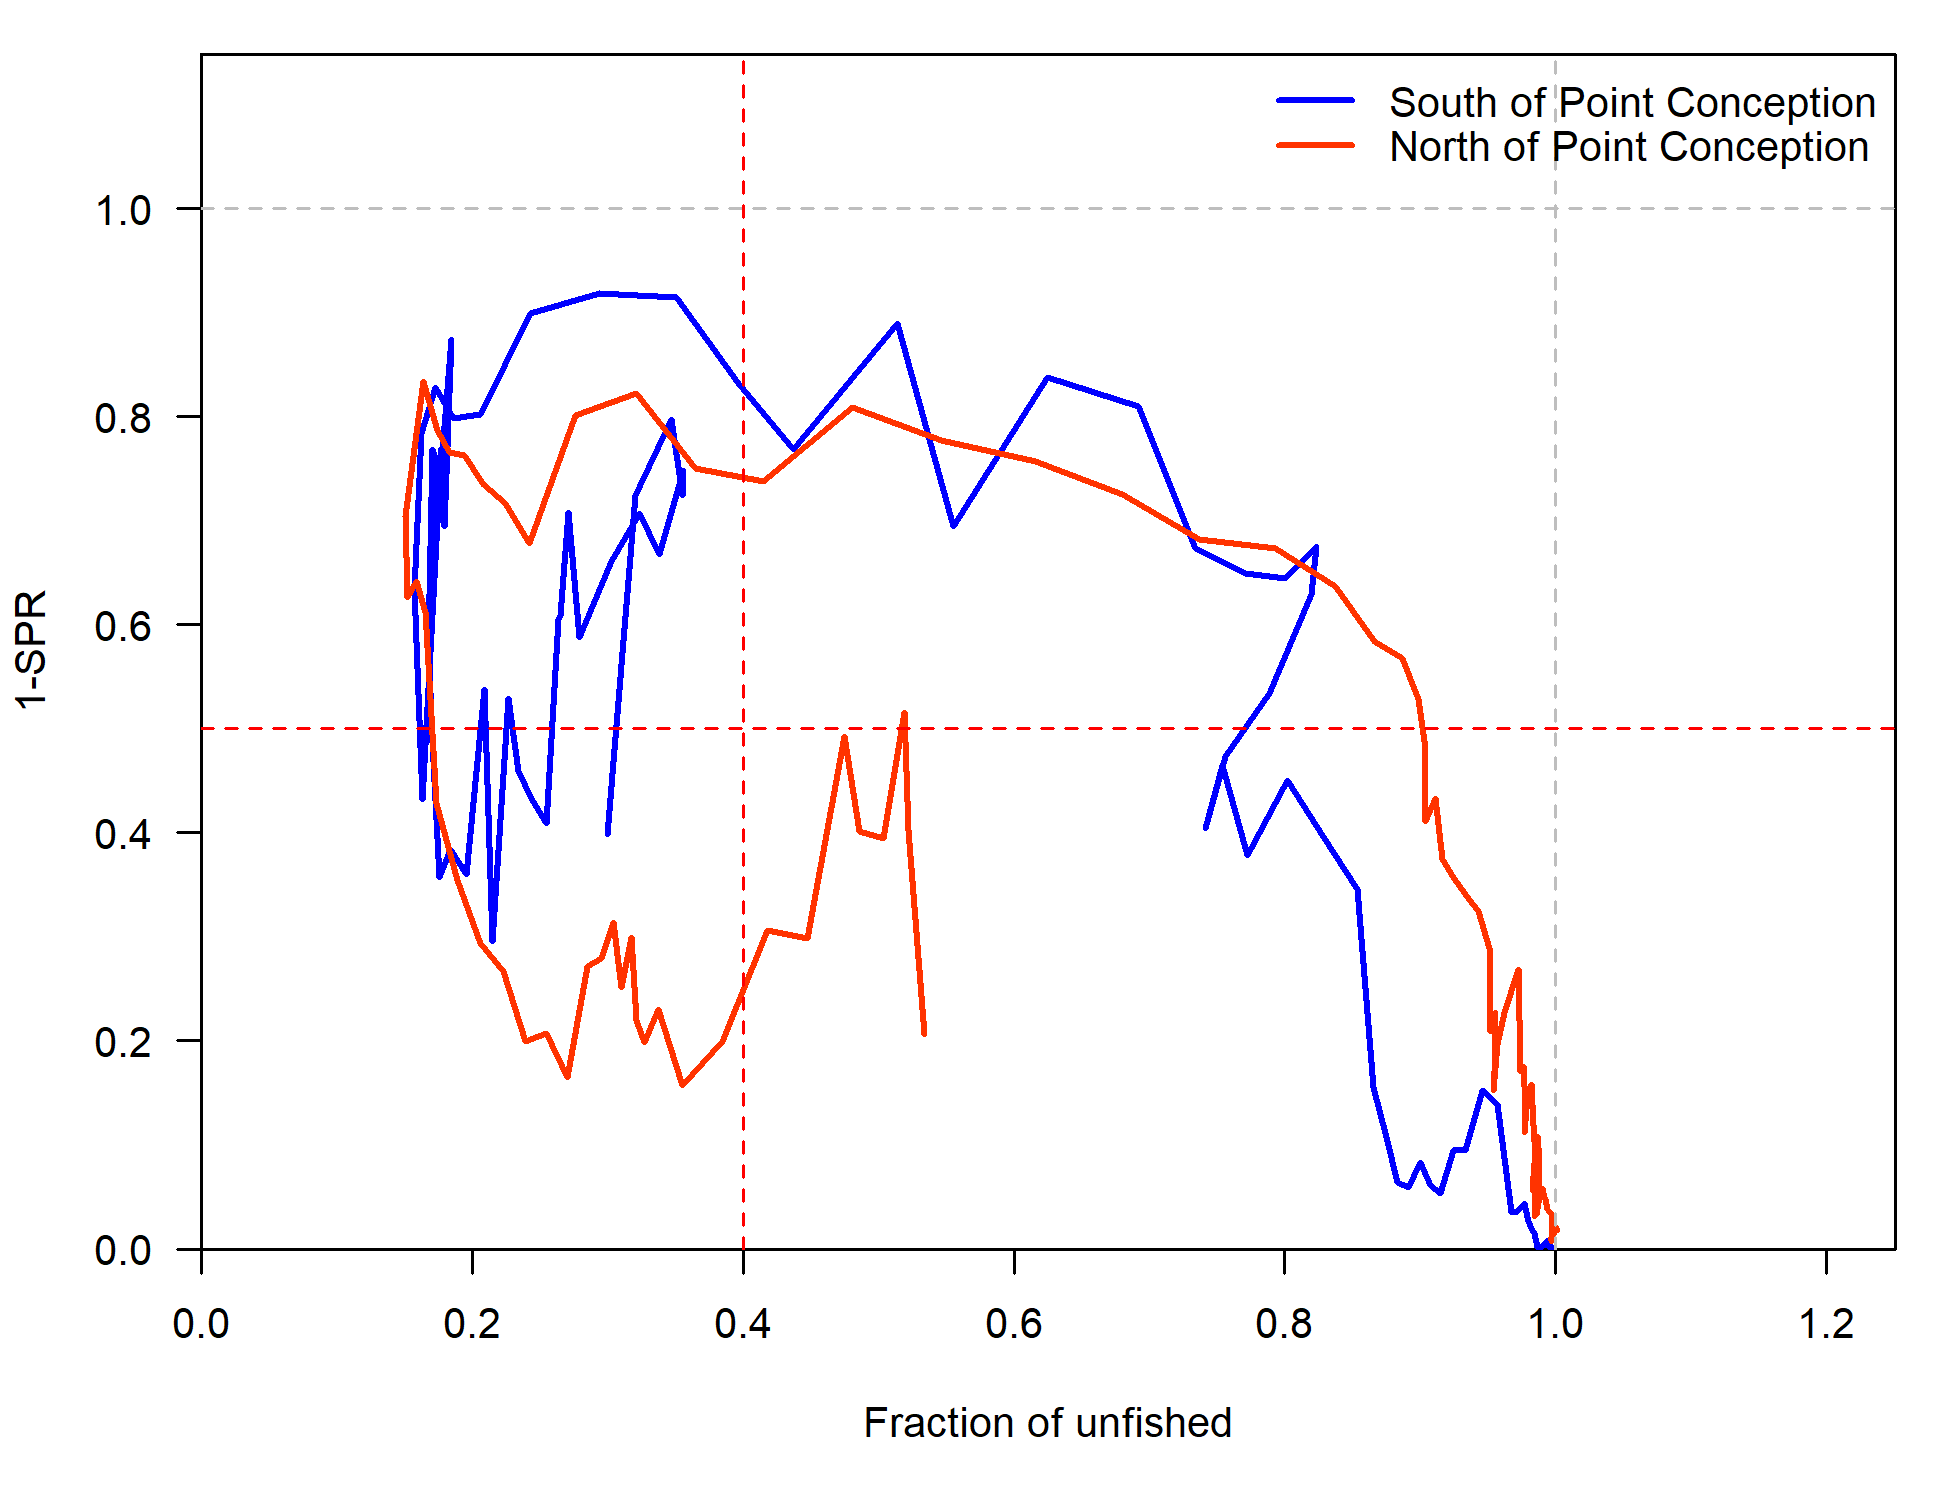
\includegraphics[alt=See Table 22 in this document and Table 15 in the north of Point Conception assessment document.,width=1\textwidth,height=1\textheight]{C:/Users/melissa.monk/Documents/GitHub/copper_rockfish_2023/documents/shared_figures/compare15_phase_plot.png}
}
\caption{Phase plot of estimated 1-SPR versus fraction unfished for the model areas south and north of Point Conception.\label{fig:es-phase}}
\end{figure}

\begin{figure}
{\centering
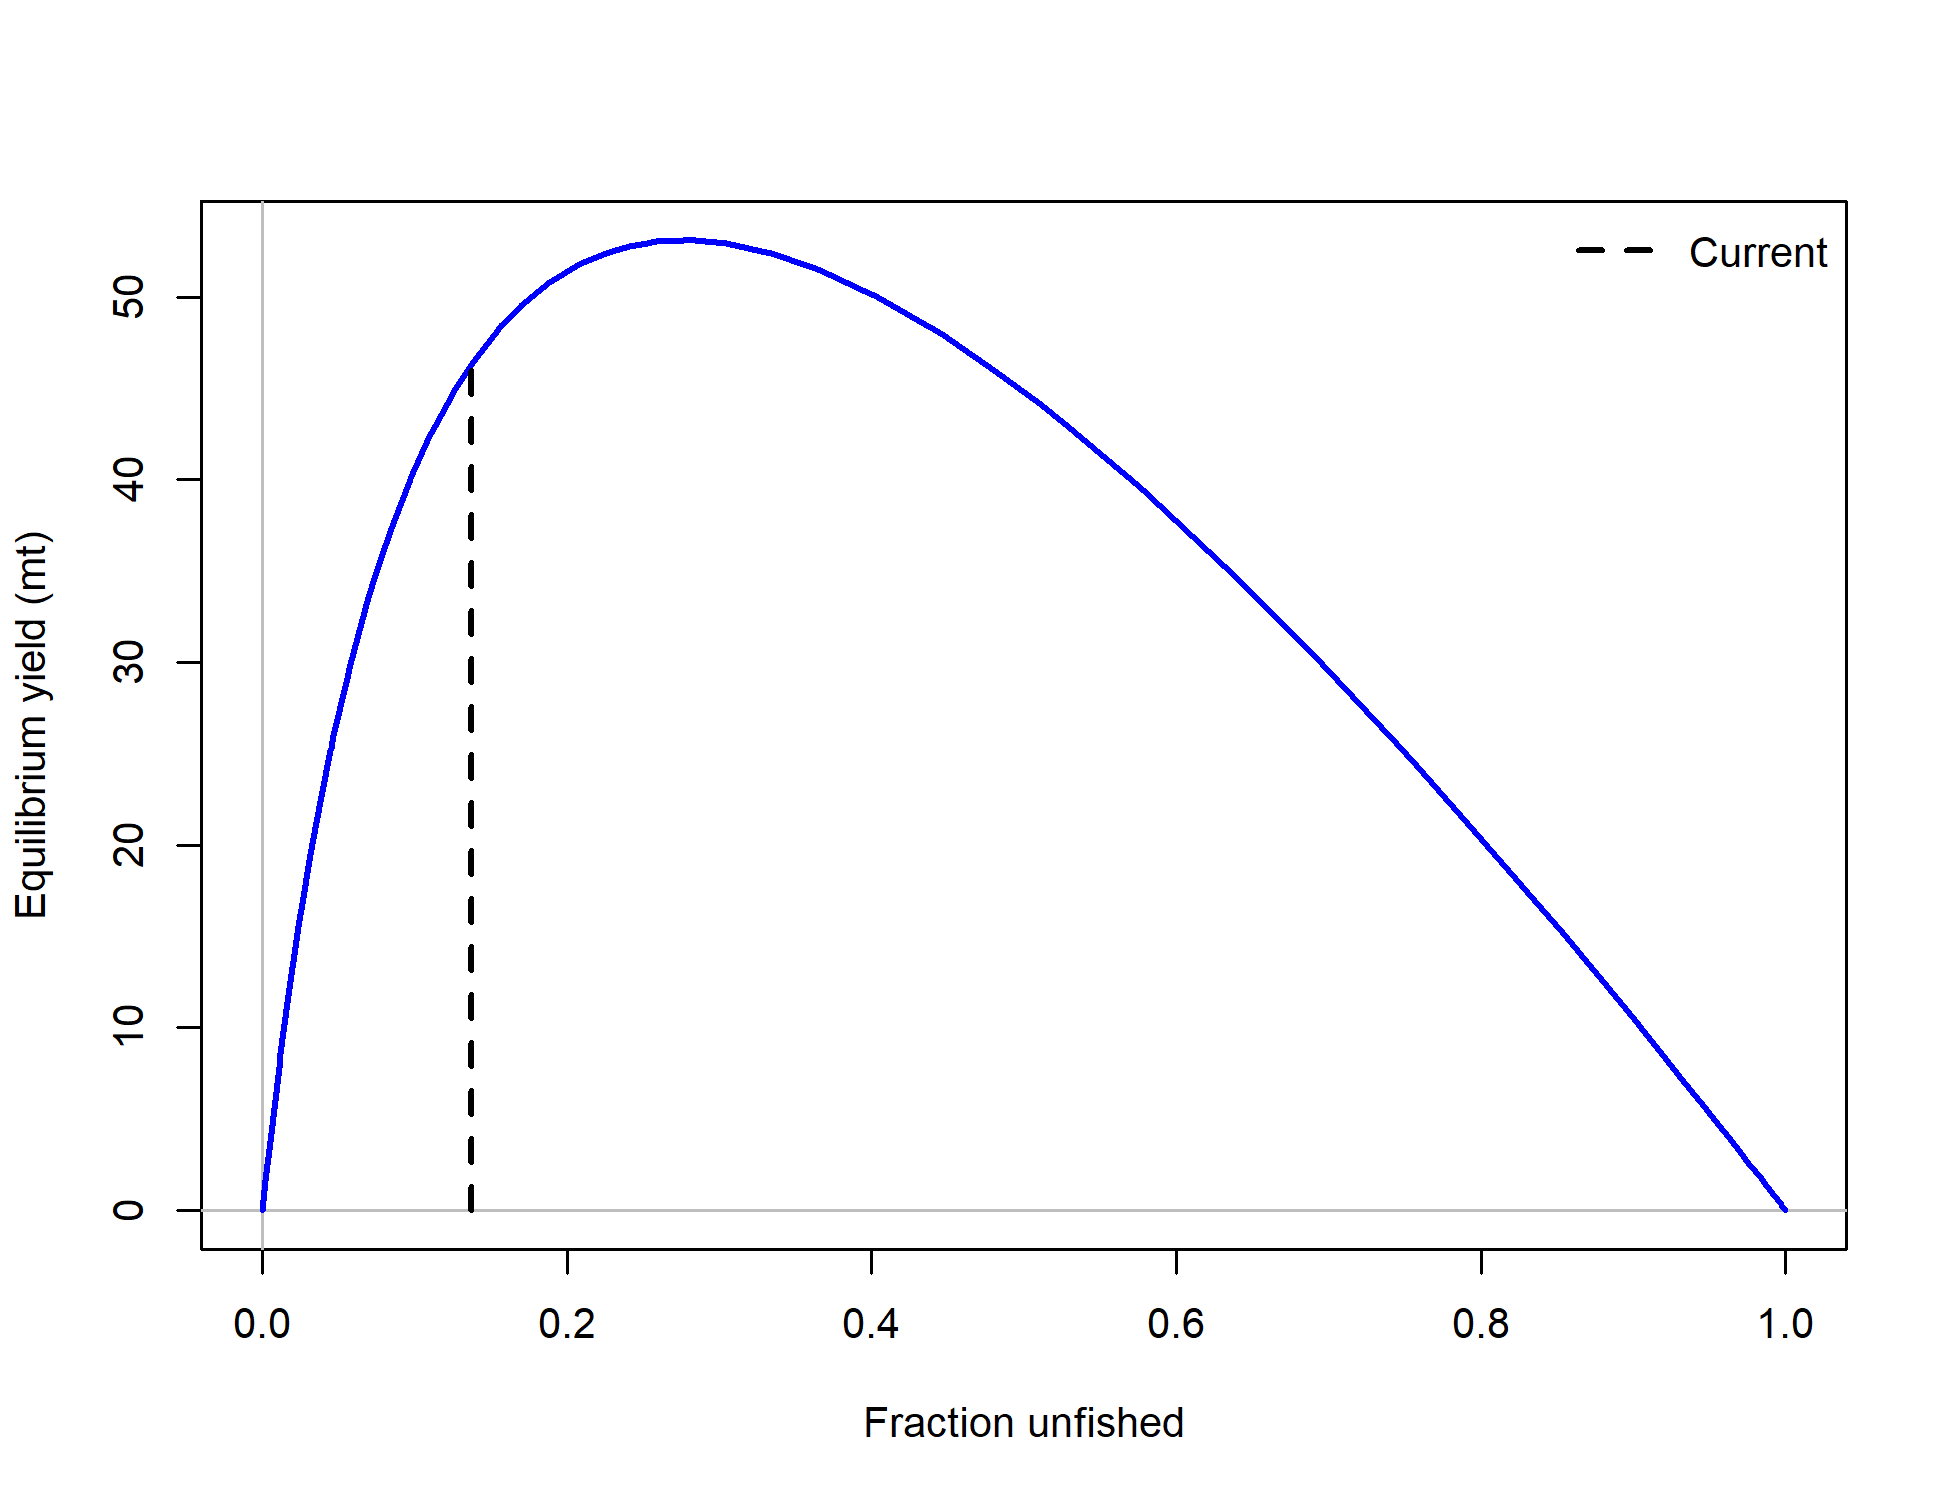
\includegraphics[alt=Equilibrium curve peaks around 0.30 fraction of unfished with the estimated current fraction of unfished at 0.16.,width=1\textwidth,height=1\textheight]{C:/Users/melissa.monk/Documents/GitHub/copper_rockfish_2023/documents/shared_figures/south_yield2_yield_curve_with_refpoints.png}
}
\caption{Equilibrium yield curve for the base case model south of Point Conception. Values are based on the 2022
fishery selectivities and with steepness fixed at 0.72.\label{fig:south-es-yield}}
\end{figure}

\begin{figure}
{\centering
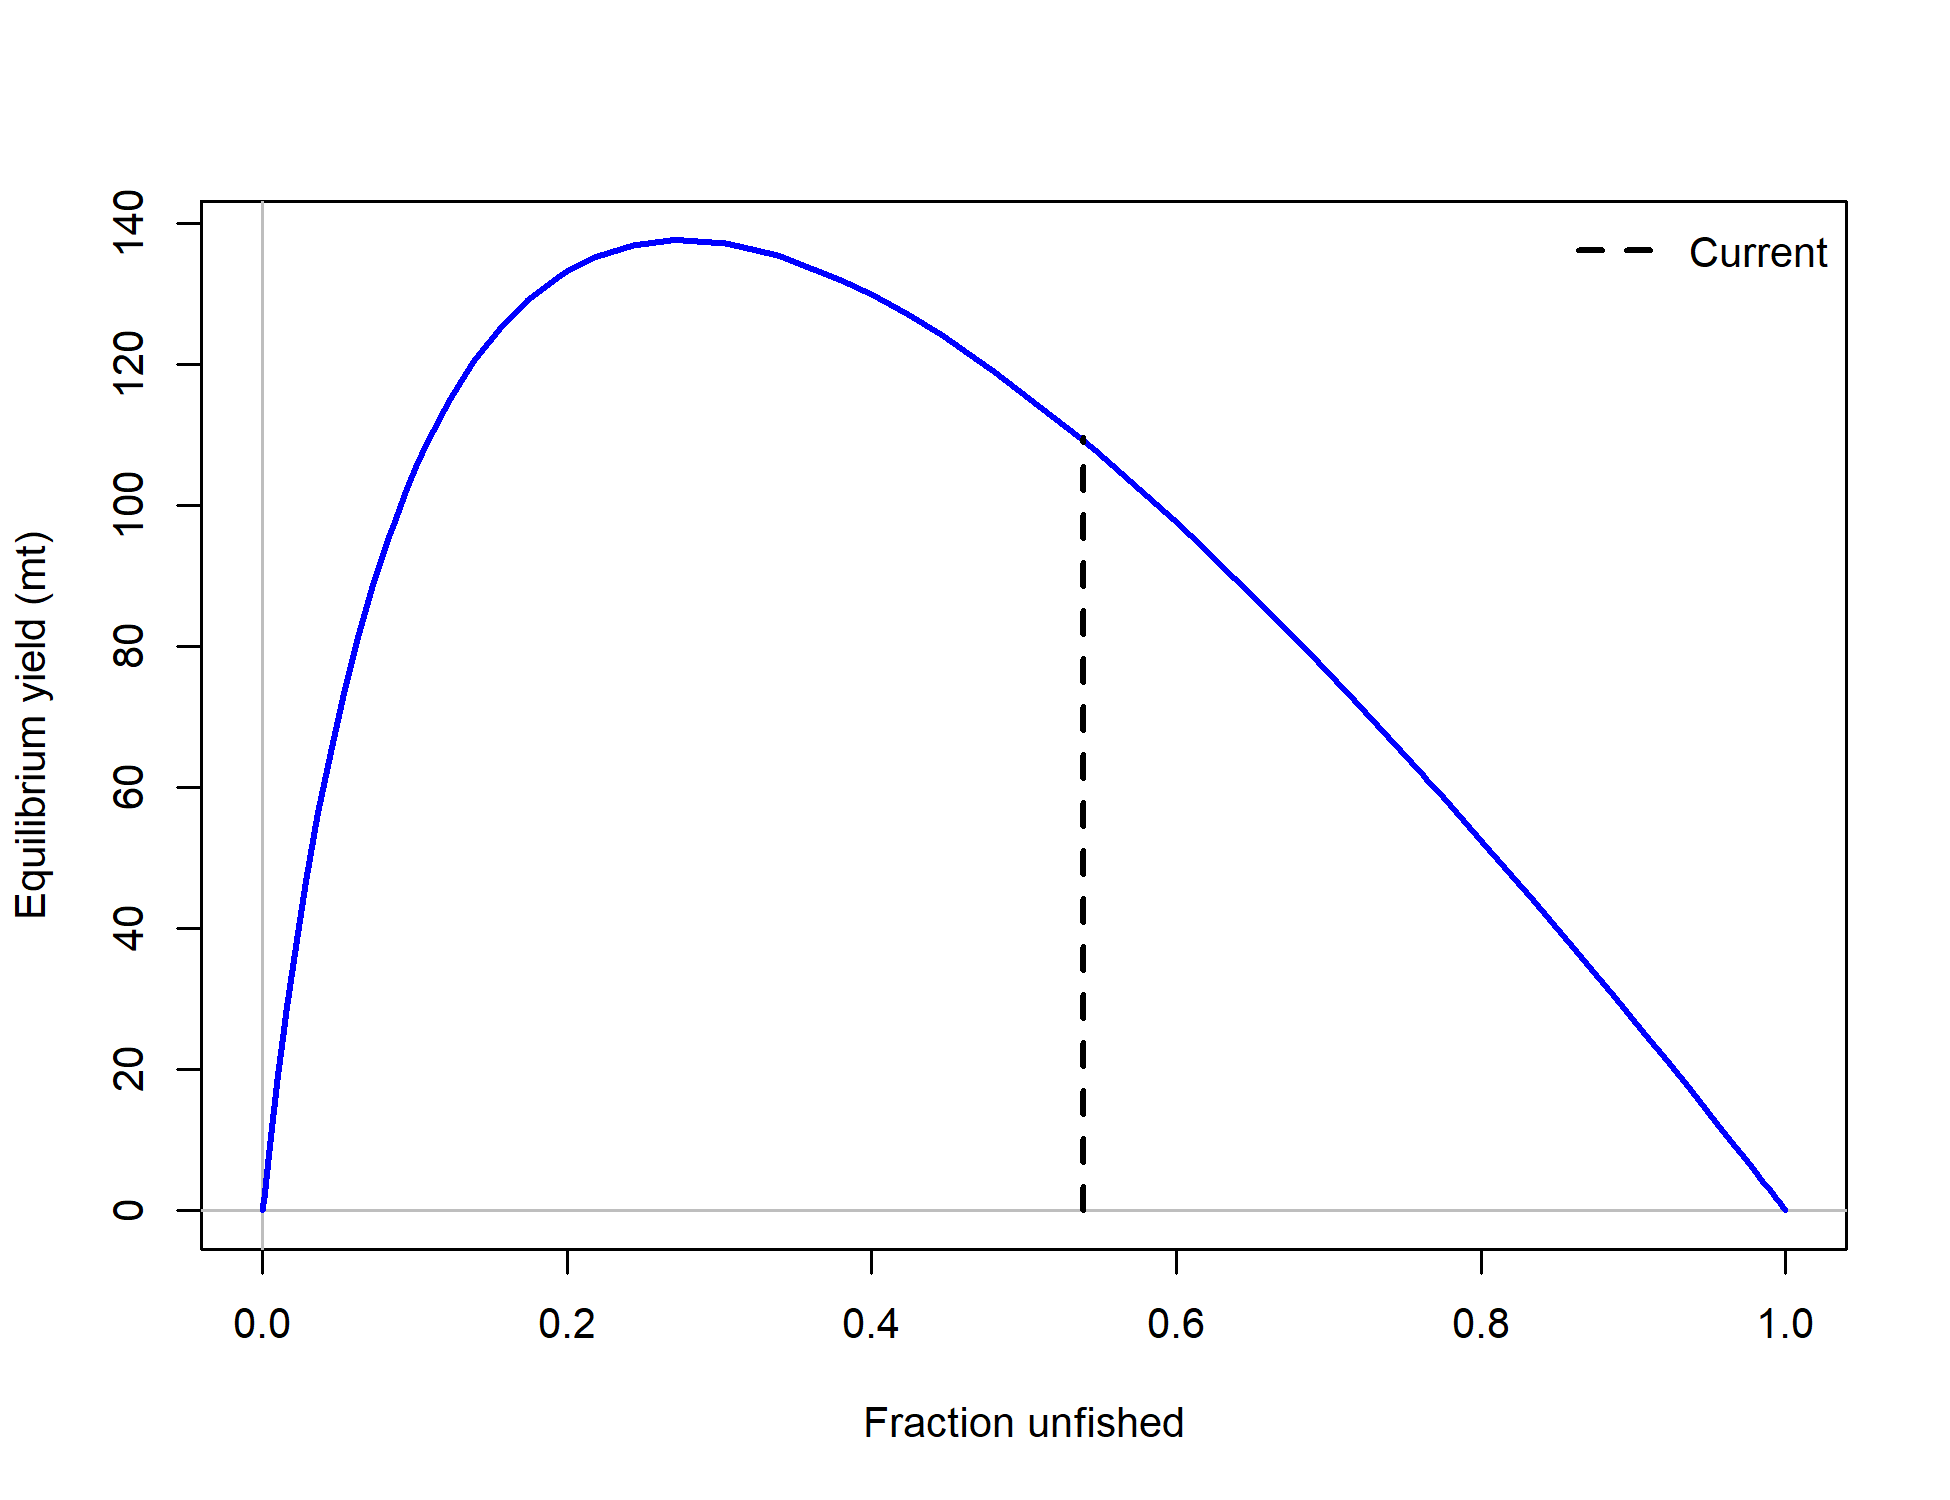
\includegraphics[alt=Equilibrium curve peaks around 0.30 fraction of unfished with the estimated current fraction of unfished at 0.46.,width=1\textwidth,height=1\textheight]{C:/Users/melissa.monk/Documents/GitHub/copper_rockfish_2023/documents/shared_figures/north_yield2_yield_curve_with_refpoints.png}
}
\caption{Equilibrium yield curve for the base case model north of Point Conception. Values are based on the 2022
fishery selectivities and with steepness fixed at 0.72.\label{fig:north-es-yield}}
\end{figure}

\pagebreak

\subsection*{Management performance}\label{management-performance}
\addcontentsline{toc}{subsection}{Management performance}

Copper rockfish are currently managed within two Nearshore Rockfish Complexes, split north and south of 40\(^\circ\) 10' N. lat. The complexes are managed based on overfishing limits (OFL) and annual catch limits (ACL) that are determined by summing the species-specific OFLs and ACLs (ACLs set equal to the Acceptable Biological Catches {[}ABCs{]}) contributions for all stocks managed in the complexes. Limits are shared among all commercial and recreational fleets with the various management procedures intended to maintain removals below the total OFL and ACL for the Nearshore Rockfish north and south complexes as a whole, rather than on a species by species basis.

The species-specific OFL and ACL contribution for copper rockfish that is allocated to California waters, Nearshore Rockfish South and 25 percent of the Nearshore Rockfish North, is shown in Table \ref{tab:es-ca-management} as well as the total catch across California. Over the last ten years the catches of copper rockfish have been below the species-specific ACLs in California. In 2021 all U.S. West Coast stocks of copper rockfish were assessed that informed the 2023-24 harvest specifications species-specific OFLs and ACLs. In California waters the new OFLs and ACLs for the 2023-24 management cycle were significantly lower than early years, resulting in in-season management action by CDFW for 2022 to reduce removals based on the latest stock assessment.

\begingroup\fontsize{10}{12}\selectfont
\begingroup\fontsize{10}{12}\selectfont

\begin{longtable}[t]{c>{\centering\arraybackslash}p{2cm}>{\centering\arraybackslash}p{2cm}>{\centering\arraybackslash}p{2cm}}
\caption{\label{tab:es-ca-management}The species-specific Overfishing Limit (OFL) and Annual Catch Limit (ACL) allocated to California and the total catch (mt) in California waters by year.}\\
\toprule
Year & OFL (mt) & ACL (mt) & Catch (mt)\\
\midrule
\endfirsthead
\caption[]{The species-specific Overfishing Limit (OFL) and Annual Catch Limit (ACL) allocated to California and the total catch (mt) in California waters by year. (\textit{continued)}}\\
\toprule
Year & OFL (mt) & ACL (mt) & Catch (mt)\\
\midrule
\endhead

\endfoot
\bottomrule
\endlastfoot
2012 & 163.2 & 136.2 & 86.0\\
2013 & 148.0 & 123.4 & 105.2\\
2014 & 148.0 & 123.4 & 98.7\\
2015 & 303.8 & 277.3 & 147.6\\
2016 & 286.9 & 262.0 & 165.3\\
2017 & 313.7 & 286.4 & 225.5\\
2018 & 319.6 & 291.8 & 203.7\\
2019 & 325.1 & 296.8 & 182.6\\
2020 & 330.4 & 301.6 & 173.4\\
2021 & 249.8 & 206.4 & 127.8\\
2022 & 249.5 & 204.0 & 66.7\\*
\end{longtable}
\endgroup{}
\endgroup{}

\subsection*{Unresolved problems and major uncertainties}\label{unresolved-problems-and-major-uncertainties}
\addcontentsline{toc}{subsection}{Unresolved problems and major uncertainties}

This assessment models the sub-areas north and south of Point Conception as separate non-mixing sub-populations, but there is likely larval or juvenile dispersal, and potentially some adult movement among these areas. Dispersal and movement rates are not well known. Improved understanding around the dispersal rates of copper rockfish across California, particularly around Point Conception, are needed to support spatial modeling of the stock.

The primary fishery-independent survey for West Coast groundfish, the Northwest Fisheries Science Center (NWFSC) West Coast Groundfish Bottom Trawl (WCGBT) survey, does not sample rocky habitats where most copper rockfish are found, and thus does not provide a robust index of abundance. An alternative survey, the CCFRP Hook and Line survey, provides a reasonable signal for copper rockfish, including relative abundance and demographic structure inside and outside a number of Marine Protect Areas (MPAs).

Age data are limited and consequently growth estimates are uncertain and the available age data contained little to no information to support the estimation of natural mortality. There is some tension among limited data sources and types inferred by the likelihood profiles, with age data suggesting a higher natural mortality rate and length data suggesting a lower value, particularly for the area north of Point Conception. Conflicting signals in the information between length and age data is commonly encountered for many West Coast groundfish stock assessments. The mechanisms driving these differences are uncertain.

Each of the sub-area models estimates high recruitment events over the most recent decade, especially relative to previous time periods. The base model for the sub-area north of Point Conception estimated overall lower variation in recruitment relative to the model south of Point Conception. Oceanographic conditions likely drive periods of either poor or above average recruitment, particularly for rockfish species. However, it is unclear what conditions may be contributing to the differing levels of recruitment variation across the California coast.

\subsection*{Decision table and projections}\label{decision-table-and-projections}
\addcontentsline{toc}{subsection}{Decision table and projections}

Both sub-area models for the California stock of copper rockfish was assigned a category 1 determination by the Scientific and Statistical Committee to the PFMC. A ten-year projection using the combined estimates from each sub-area base model, south and north of Point Conception in California, with catches equal to the estimated Annual Catch Limit (ACL) based on the category 1 time-varying \(\sigma\) with \(P^*\) = 0.45 for years 2025-2034 is shown in Table \ref{tab:es-ca-proj} (i.e., termed the ``buffer''). The removals in 2023 and 2024 were set equal to the portion of copper rockfish species-specific adopted ACLs for California determined by summing the adopted ACLs south of $40^\circ 10^\prime$ N. lat. and the portion of the north of $40^\circ 10^\prime$ N. lat. allocated to California (25 percent - PFMC Groundfish Management Team pers. comm.). The portion of ACL to allocate to each sub-area for 2023-24 was determined based on the proportion of the total removals by area in 2022 (71 percent north and 29 percent south) as recommended by the GMT (Mel Mandrup, CDFW, personal communication). The projections were conducted in an iterative fashion based on the combined estimates of spawning output, relative spawning output, OFL, ABC, and ACL for each year. The estimated proportion of the ACL removed from each sub-area model was based on the proportion of the contribution to the total annual OFL estimate. The allocation of the OFL, ABC, and ACL north and south of $40^\circ 10^\prime$ N. lat. based on the estimates of rocky habitat and the density of copper rockfish in the area are given in Table \ref{tab:es-ca-proj-split}.

At the end of the projection period, 2034, the projected ACL removals result in the California stock increasing to be above the biomass target at percent of the relative spawning output, with the portion of the stock south at 24.5 percent of the sub-area estimated relative spawning output and north of Point Conception at 48.2 percent.

The axes of uncertainty in the decision table are based on the uncertainty around steepness. The estimated uncertainty around the 2023 OFL was used to identify the low and high states of nature that would align with the 12.5 and 87.5 percentiles from the base model where the base model is assigned a 50 percent probability of being the true state of nature and both the low and high states of nature being assigned a 25 percent probability. A search across steepness (\(h\)) values for each sub-area model was conducted to identify the corresponding steepness values that would create the low and high states of nature relative to the base model. The sub-area north of Point Conception applied values of \(h\) of: 0.655, 0.72, and 0.859. The sub-area south of Point Conception applied values of \(h\) of: 0.54, 0.72, and 0.929. The proposed decision table assumes full ACL removal during the projection period under P* alternative catch stream (Table \ref{tab:dec-tab-es}).

\begingroup\fontsize{9}{11}\selectfont

\begin{landscape}\begingroup\fontsize{9}{11}\selectfont

\begin{longtable}[t]{c>{\centering\arraybackslash}p{1.3cm}>{\centering\arraybackslash}p{1.1cm}>{\centering\arraybackslash}p{1.1cm}>{\centering\arraybackslash}p{1.1cm}>{\centering\arraybackslash}p{1.1cm}>{\centering\arraybackslash}p{1.4cm}>{\centering\arraybackslash}p{1.4cm}>{\centering\arraybackslash}p{1.6cm}>{\centering\arraybackslash}p{1.6cm}>{\centering\arraybackslash}p{1.3cm}}
\caption{\label{tab:es-ca-proj}The estimated OFL (mt), ABC (mt), ACL (mt), buffer, spawning output in billions of eggs across California, and relative spawning outut by year along with the sub-area allocations of the ACL south of Point Conception (south, $34^\circ 27^\prime$ N. lat.), north of Point Conception to $40^\circ 10^\prime$ N. lat. (central), and $40^\circ 10^\prime$ to $42^\circ$ N. lat. (north).}\\
\toprule
Year & Assumed Catch (mt) & OFL (mt) & ABC (mt) & ACL (mt) & Buffer & Spawning Output & Fraction Unfished & Sub-ACL South (mt) & Sub-ACL Central (mt) & Sub-ACL North (mt)\\
\midrule
\endfirsthead
\caption[]{The estimated OFL (mt), ABC (mt), ACL (mt), buffer, spawning output in billions of eggs across California, and relative spawning outut by year along with the sub-area allocations of the ACL south of Point Conception (south, $34^\circ 27^\prime$ N. lat.), north of Point Conception to $40^\circ 10^\prime$ N. lat. (central), and $40^\circ 10^\prime$ to $42^\circ$ N. lat. (north). (\textit{continued)}}\\
\toprule
Year & Assumed Catch (mt) & OFL (mt) & ABC (mt) & ACL (mt) & Buffer & Spawning Output & Fraction Unfished & Sub-ACL South (mt) & Sub-ACL Central (mt) & Sub-ACL North (mt)\\
\midrule
\endhead

\endfoot
\bottomrule
\endlastfoot
2023 & 91.5 & - & - & - & - & 240.80 & 0.366 & - & - & -\\
2024 & 94.7 & - & - & - & - & 245.88 & 0.374 & - & - & -\\
2025 & - & 143.5 & 134.1 & 131.9 & 0.935 & 250.60 & 0.381 & 15.8 & 109.2 & 6.8\\
2026 & - & 145.3 & 135.2 & 133.1 & 0.93 & 251.62 & 0.383 & 18 & 108.4 & 6.7\\
2027 & - & 147.2 & 136.3 & 134.5 & 0.926 & 252.91 & 0.385 & 20.1 & 107.7 & 6.7\\
2028 & - & 148.9 & 137.3 & 135.8 & 0.922 & 254.64 & 0.388 & 22 & 107.1 & 6.7\\
2029 & - & 150.4 & 137.9 & 136.7 & 0.917 & 256.75 & 0.391 & 23.5 & 106.6 & 6.6\\
2030 & - & 151.6 & 138.5 & 137.7 & 0.913 & 259.10 & 0.394 & 24.8 & 106.3 & 6.6\\
2031 & - & 152.8 & 138.9 & 138.6 & 0.909 & 261.54 & 0.398 & 26 & 106 & 6.6\\
2032 & - & 153.9 & 139.1 & 139.1 & 0.904 & 264.02 & 0.402 & 27 & 105.6 & 6.6\\
2033 & - & 155 & 139.5 & 139.5 & 0.9 & 266.52 & 0.406 & 27.9 & 105.1 & 6.5\\
2034 & - & 156.2 & 139.9 & 139.9 & 0.896 & 269.04 & 0.409 & 28.8 & 104.6 & 6.5\\*
\end{longtable}
\endgroup{}
\end{landscape}
\endgroup{}

\pagebreak

'

\begingroup\fontsize{10}{12}\selectfont
\begingroup\fontsize{10}{12}\selectfont

\begin{longtable}[t]{c>{\centering\arraybackslash}p{1.3 cm}>{\centering\arraybackslash}p{1.3 cm}>{\centering\arraybackslash}p{1.3 cm}>{\centering\arraybackslash}p{1.3 cm}>{\centering\arraybackslash}p{1.3 cm}>{\centering\arraybackslash}p{1.3 cm}>{\centering\arraybackslash}p{1.3 cm}}
\caption{\label{tab:es-ca-proj-split}The estimated California OFL (mt), ABC (mt), and ACL (mt) split south and north $40^\circ 10^\prime$ N. lat. The estimated percent allocated to the north $40^\circ 10^\prime$ N. lat. in California is 5.86 percent based on estimates of rocky habitat and density of copper rockfish in the area.}\\
\toprule
Year & Assumed Catch (mt) & South OFL (mt) & South ABC (mt) & South ACL (mt) & North OFL (mt) & North ABC (mt) & North ACL (mt)\\
\midrule
\endfirsthead
\caption[]{The estimated California OFL (mt), ABC (mt), and ACL (mt) split south and north $40^\circ 10^\prime$ N. lat. The estimated percent allocated to the north $40^\circ 10^\prime$ N. lat. in California is 5.86 percent based on estimates of rocky habitat and density of copper rockfish in the area. (\textit{continued)}}\\
\toprule
Year & Assumed Catch (mt) & South OFL (mt) & South ABC (mt) & South ACL (mt) & North OFL (mt) & North ABC (mt) & North ACL (mt)\\
\midrule
\endhead

\endfoot
\bottomrule
\endlastfoot
2023 & 91.5 & - & - & - & - & - & -\\
2024 & 94.7 & - & - & - & - & - & -\\
2025 & - & 136.06 & 127.22 & 125.08 & 7.4 & 6.92 & 6.8\\
2026 & - & 137.97 & 128.31 & 126.33 & 7.37 & 6.85 & 6.75\\
2027 & - & 139.91 & 129.55 & 127.79 & 7.34 & 6.8 & 6.7\\
2028 & - & 141.63 & 130.58 & 129.11 & 7.32 & 6.74 & 6.67\\
2029 & - & 143.09 & 131.21 & 130.1 & 7.3 & 6.69 & 6.64\\
2030 & - & 144.36 & 131.8 & 131.1 & 7.28 & 6.65 & 6.61\\
2031 & - & 145.53 & 132.28 & 131.99 & 7.28 & 6.61 & 6.6\\
2032 & - & 146.65 & 132.57 & 132.57 & 7.27 & 6.57 & 6.57\\
2033 & - & 147.77 & 132.99 & 132.99 & 7.27 & 6.54 & 6.54\\
2034 & - & 148.92 & 133.43 & 133.43 & 7.27 & 6.51 & 6.51\\*
\end{longtable}
\endgroup{}
\endgroup{}

\pagebreak

\begingroup\fontsize{9}{11}\selectfont
\begingroup\fontsize{9}{11}\selectfont

\begin{longtable}[t]{l>{\raggedright\arraybackslash}p{0.8cm}>{\raggedright\arraybackslash}p{0.8cm}>{\raggedright\arraybackslash}p{1.45cm}>{\raggedright\arraybackslash}p{1.45cm}>{\raggedright\arraybackslash}p{1.45cm}>{\raggedright\arraybackslash}p{1.45cm}>{\raggedright\arraybackslash}p{1.45cm}>{\raggedright\arraybackslash}p{1.45cm}}
\caption{\label{tab:dec-tab-es}Decision table summary of 10-year projections beginning in 2025 for alternative states of nature based on an axis of uncertainty around steepness for both California sub-area models. The spawning output and depletion is for the whole California stock with the annual projected catch removed from each sub-area model equal to the contribution proportion for each sub-area OFL. Columns range over low, mid, and high states of nature and rows range over different catch P* values. The removals in 2023 and 2025 are set equal to the adopted ACL for the California stock.}\\
\toprule
\multicolumn{3}{c}{ } & \multicolumn{2}{c}{Low Steepness} & \multicolumn{2}{c}{Base Steepness} & \multicolumn{2}{c}{High Steepness} \\
\cmidrule(l{3pt}r{3pt}){4-5} \cmidrule(l{3pt}r{3pt}){6-7} \cmidrule(l{3pt}r{3pt}){8-9}
  & Year & Catch & Spawning Output & Fraction Unfished & Spawning Output & Fraction Unfished & Spawning Output & Fraction Unfished\\
\hline
&	2023	&	91.5	&	176.2	&	0.255	&	240.8	&	0.366	&	337.3	&	0.533	\\
&	2024	&	94.7	&	178.2	&	0.258	&	245.9	&	0.374	&	345.7	&	0.546	\\
&	2025	&	131.9	&	180.2	&	0.261	&	250.6	&	0.381	&	352.9	&	0.558	\\
&	2026	&	133.1	&	178.9	&	0.259	&	251.6	&	0.382	&	355.4	&	0.562	\\
&	2027	&	134.5	&	178.2	&	0.258	&	252.9	&	0.384	&	357.3	&	0.564	\\
ACL	&	2028	&	135.8	&	178.0	&	0.258	&	254.6	&	0.387	&	358.9	&	0.567	\\
P* 0.45	&	2029	&	136.7	&	178.3	&	0.258	&	256.7	&	0.390	&	360.4	&	0.569	\\
&	2030	&	137.7	&	178.9	&	0.259	&	259.1	&	0.394	&	361.8	&	0.572	\\
&	2031	&	138.6	&	179.6	&	0.260	&	261.5	&	0.397	&	363.1	&	0.574	\\
&	2032	&	139.1	&	180.4	&	0.261	&	264.0	&	0.401	&	364.3	&	0.575	\\
&	2033	&	139.5	&	181.2	&	0.262	&	266.5	&	0.405	&	365.3	&	0.577	\\
&	2034	&	139.9	&	182.0	&	0.264	&	269.0	&	0.409	&	366.2	&	0.578	\\
\hline																	
&	2023	&	91.5	&	176.2	&	0.255	&	240.8	&	0.366	&	337.3	&	0.533	\\
&	2024	&	94.7	&	178.2	&	0.258	&	245.9	&	0.374	&	345.7	&	0.546	\\
&	2025	&	123.1	&	180.2	&	0.261	&	250.6	&	0.381	&	352.9	&	0.558	\\
&	2026	&	124.2	&	179.7	&	0.260	&	252.4	&	0.384	&	356.3	&	0.563	\\
&	2027	&	125.4	&	179.9	&	0.261	&	254.6	&	0.387	&	359.1	&	0.567	\\
ACL	&	2028	&	126.5	&	180.7	&	0.262	&	257.3	&	0.391	&	361.6	&	0.571	\\
P* 0.40	&	2029	&	127.4	&	181.9	&	0.263	&	260.3	&	0.396	&	364.1	&	0.575	\\
&	2030	&	128.1	&	183.4	&	0.266	&	263.6	&	0.401	&	366.4	&	0.579	\\
&	2031	&	128.2	&	185.1	&	0.268	&	267.1	&	0.406	&	368.7	&	0.582	\\
&	2032	&	128.4	&	186.9	&	0.271	&	270.6	&	0.411	&	370.8	&	0.586	\\
&	2033	&	128.4	&	188.8	&	0.273	&	274.1	&	0.416	&	372.8	&	0.589	\\
&	2034	&	128.5	&	190.7	&	0.276	&	277.7	&	0.422	&	374.7	&	0.592	\\
\hline																	
&	2023	&	91.5	&	176.2	&	0.255	&	240.8	&	0.366	&	337.3	&	0.533	\\
&	2024	&	94.7	&	178.2	&	0.258	&	245.9	&	0.374	&	345.7	&	0.546	\\
&	2025	&	114.7	&	180.2	&	0.261	&	250.6	&	0.381	&	352.9	&	0.558	\\
&	2026	&	115.6	&	180.5	&	0.261	&	253.3	&	0.385	&	357.1	&	0.564	\\
ACL	&	2027	&	116.7	&	181.5	&	0.263	&	256.3	&	0.389	&	360.7	&	0.570	\\
P* 0.35	&	2028	&	117.5	&	183.2	&	0.265	&	259.8	&	0.395	&	364.2	&	0.575	\\
&	2029	&	118.2	&	185.3	&	0.268	&	263.8	&	0.401	&	367.6	&	0.581	\\
&	2030	&	118.1	&	187.8	&	0.272	&	268.1	&	0.407	&	370.9	&	0.586	\\
&	2031	&	118.0	&	190.5	&	0.276	&	272.5	&	0.414	&	374.1	&	0.591	\\
&	2032	&	117.9	&	193.4	&	0.280	&	277.0	&	0.421	&	377.2	&	0.596	\\
&	2033	&	117.6	&	196.3	&	0.284	&	281.5	&	0.428	&	380.2	&	0.601	\\
&	2034	&	117.4	&	199.2	&	0.289	&	286.1	&	0.435	&	383.1	&	0.605	\\*
 \hline
\end{longtable}
\endgroup{}
\endgroup{}


\pagebreak

\subsection*{Scientific uncertainty}\label{scientific-uncertainty}
\addcontentsline{toc}{subsection}{Scientific uncertainty}

The model estimated uncertainty around the 2023 spawning output for the sub-area model south of Point Conception is \(\sigma\) = 0.3 and the uncertainty for the sub-area model north of Point Conception is \(\sigma\) = 0.31. The uncertainty around the OFL south and north of Point Conception was \(\sigma\) = 0.28 and 0.3, respectively. Each of these are likely underestimates of overall uncertainty due to the necessity to fix several key population dynamics parameters (e.g., steepness, recruitment variance, natural mortality) and also because there is no explicit incorporation of model structural uncertainty (although see the decision table for alternative states of nature).

\subsection*{Research and data needs}\label{research-and-data-needs}
\addcontentsline{toc}{subsection}{Research and data needs}

There were some major sources of uncertainty within the assessments for copper rockfish. To improve our understanding of the copper rockfish stock in California waters the following research and data collection should be prioritized:

\begin{enumerate}

    \item  The NWFSC Hook and Line survey is the only long-term fishery-independent survey in rocky (untrawlable) habitat in the Southern California Bight. Efforts should continue to explore how best to model hook and line catch data to develop indices of abundance. We also recommend evaluating how to structure the NWFSC Hook and Line survey index, given its expansion into the CCAs and increase in sites within designated MPAs, and independent analysis of information content in NWFSC Hook and Line survey across observed species. Finally, increased spatiotemporal sampling around Point Conception would aid in identifying stock boundaries.

    \item The assessment area south of Point Conception appears to have a mixture of observations from areas experiencing variable fishing mortality. In the region there are likely a mixture of areas: open access rocky reefs that are close to port that are heavily fished, open access rocky reefs that are inaccessible via day-trips that are fished but likely at lower levels, and rocky reefs that fall within marine protected areas (MPAs). A spatially-explicit assessment model may be able to capture this complexity but will require data (indices of abundance and composition data) from each of the regions. 
    
    \item Future nearshore assessments would greatly benefit from additional CDFW ROV surveys which could increase the power of these data to inform assessments.

    \item There are very limited age data for copper rockfish across California arising from fishery-dependent sources. Establishing regular collections of otoliths from the recreational fishery, a large source of mortality, would support future assessments and would improve the understanding of the population structure and life history of copper rockfish. 

    \item There is limited information for copper rockfish on maturity and fecundity and the variability of these parameters with increasing latitude.  The NWFSC WCGBT and Hook and Line surveys provided the only available information on the maturity ogive and the timing of these surveys does not overlap with the expected peak spawning season. The Southwest Fisheries Science Center has egg samples from a total of ten copper rockfish, which is too few to draw conclusions regarding fecundity.

    \item Some of the PR mode recreational data that should be available via RecFIN were found to contain information in that database inconsistent with datasheets available from CDFW. There is also a question if length data collected by the Deb Wilson-Vandenberg onboard observer survey is duplicated within RecFIN and attributed to MRFSS dockside samples of the CPFV fleet.

    \item The interpreted substrate data for the areas north of Point Conception within state waters is incomplete. Additional data needs include high resolution interpreted substrate maps for areas outside of state waters. The available interpreted bathymetry data from south of Point Conception is incomplete within state waters  around the northern and southern Channel Islands. This poses a challenge for estimating available rocky substrate both by district and also inside and outside closed areas. 

    \item The genetic stock structure of copper rockfish warrants further investigation to ensure appropriate management of copper rockfish along the West Coast. 

    \item The Marine Recreational Fisheries Statistics Survey (MRFSS) index was excluded from both California assessment models. The standardized trends in abundance were marked by extreme peaks in the data throughout the time series. The STAT was unable to identify what may driving extreme changes fishing behavior in these select years. These data should be reviewed to better understand whether these data reflect true changes in fishing behavior in those years or errors in data collection. 

    \item Additional research on the effect of the MPA network on copper rockfish and other nearshore rockfish species needs to be conducted. The trend inside the MPAs in northern California exhibited an increasing trend compared to outside the MPAs, similar to what was observed during the 2021 assessment of vermilion/sunset rockfish. However, the trends inside MPAs south of Point Conception varied by location with a number of sites showing flat or declining trends.  

    \item Further investigations of other available fishery-independent data such as the Partnership for Interdisciplinary Studies of Coastal Oceans (PISCO) kelp forest index would benefit future assessments of nearshore species, including copper rockfish. 

    \item Larval and smaller young-of-the-year copper rockfish can only be identified with certainty genetically. Existing sources of data (CalCOFI and Standard Monitoring Units for the Recruitment of Fishes [SMURFs]) where genetic samples can be analyzed would provide key information to inform spawning output estimates for copper rockfish.
 
    \item Continue to improve historical catch reconstructions, including attempting to quantify uncertainty with these and other historical data.
  
    \item Existing catch estimates within Recreational Fisheries Information Network (RecFIN) that are currently assigned only to "rockfish, general" should be investigated to determine if these removals can be assigned to specific species.

\end{enumerate}

\section{Introduction}\label{introduction}

This assessment report describes the sub-area population of copper rockfish (\emph{Sebastes caurinus}) off the California coast north of Point Conception in U.S. waters, using data through 2022 (Figure \ref{fig:ca-map}). The sub-area population south of Point Conception in California waters was also evaluated and is described in a separate assessment report. The copper rockfish status for the California stock is determined by the combined estimates of spawning output from both sub-areas and is detailed in the \hyperref[management]{management} Section. This assessment does not account for populations located in Mexican waters or other areas off the U.S. West Coast and assumes that these southern and northern populations do not contribute to nor take from the population being assessed here.

\subsection{Basic Information and Life History}\label{basic-information-and-life-history}

Copper rockfish have historically been a part of both commercial and recreational fisheries throughout its range. Copper rockfish are a demersal, relatively nearshore species within the subgenus \emph{Pteropodus.} The core range of copper rockfish is comparatively large, ranging from northern Baja Mexico to the Gulf of Alaska, with copper rockfish also found in Puget Sound. Copper rockfish range from the sub-tidal (as juveniles) to depths of around 180 m {[}@love\_rockfishes\_2002{]}. Copper rockfish are commonly found in waters less than 100 m in depth inhabiting nearshore kelp forests and complex low-relief rocky habitat {[}@love\_probably\_1996{]}. Adult copper rockfish have high site fidelity and are thought to not make long-range movements. An acoustic telemetry study displaced copper rockfish 4 km from their capture location to an artificial reef and within 10 days, half of the copper rockfish returned to the original capture location {[}@reynolds\_application\_2010{]}.

Copper rockfish have a clearly defined long white band the posterior two-thirds of the lateral line. Copper rockfish have high variation in coloration throughout its range, taking on coloration from dark brown, olive, orange-red and pink, with patches of yellow and pink {[}@miller\_guide\_1972{]}. In general, the copper rockfish towards the northern part of the range are often darker in color than fish encountered in southern California. The distinct change in coloration resulted in copper rockfish initially being described as two separate species, copper rockfish (\emph{S. caurinus}) and whitebelly rockfish (\emph{S. vexillaris}).

The \emph{Sebastes} genus is viviparous with internal fertilization, many species exhibit dimorphic growth with females larger at size-at-age than males, and a number of species have reproductive strategies that vary with latitude. There are very few fecundity samples from copper rockfish available from California, although copper rockfish are assumed to produce a single brood annually during the winter months.

The pelagic larvae are encountered in the California Cooperative Oceanic Fisheries Investigations (CalCOFI) surveys, but neither larval nor young-of-the-year can be identified visually {[}@thompson\_larval\_2017{]}. The size at birth ranges from 5-6 mm and the larvae remain pelagic until approximately 22-23 mm standard length at which time they recruit to the kelp forest canopy {[}@anderson\_identification\_1983{]}.

Juvenile copper rockfish are indistinguishable from kelp (\emph{S. atrovirens}), black-and-yellow (\emph{S. chrysomelas}), and gopher (\emph{S. carnatus}) rockfishes, all of which recruit to the kelp forest canopy in the spring months. Copper rockfish is the first of the species group to recruit to the kelp forest from April to May and can be distinguished from the other species once it reaches a size around 5 cm standard length {[}@anderson\_identification\_1983{]}. @baetscher\_dispersal\_2019 genetically identified young-of-the-year rockfish from surveys in Carmel and Monterey Bays in California and provided the authors with the length and genotyped species identifications from her study. The average total length of young-of-the-year copper rockfish in July was 3-4 cm (Figure \ref{fig:copper-smurf-length}). @anderson\_identification\_1983 observed benthic copper rockfish nocturnally active over sandy bottom outside the kelp forest.

Copper rockfish are a relatively long-lived rockfish, estimated to live at least 50 years {[}@love\_probably\_1996{]}. Copper rockfish were determined to have the highest vulnerability (V = 2.27) of any West Coast groundfish stock evaluated in a productivity susceptibility analysis {[}@cope\_approach\_2011{]}. This analysis calculated species-specific vulnerability scores based on two dimensions: productivity characterized by the life history and susceptibility that characterized how the stock could be impacted by fisheries and other activities.

Copper rockfish are opportunistic carnivores and commonly consume crustaceans, mollusks, and fish whole {[}@lea\_biological\_1999; @bizzarro\_diet\_2017{]}. @prince\_food\_1972 observed a shift in a diet dominated by arthropods in age 0 and 1 fish to a more diverse diet including molluscs and fish as they aged. The study also noted that juvenile copper rockfish were preyed upon by harbor seals and lingcod. Two tagging studies of copper rockfish indicated that most individuals have a small home range, with 91 percent of recaptures from CCFRP (unpublished data) and 49 percent of individuals from @hanan\_longterm\_2012 within 1 km (straight line distance) of the original release site. Of the 117 recaptures from @hanan\_longterm\_2012, four traveled greater than 50 km, with a maximum distance of 488 km (1,222 days at liberty), and four individuals crossed the biogeographic boundary of Point Conception. Of the 133 copper rockfish recaptures from CCFRP, four traveled greater than 50 km, and the maximum distance traveled was 169 km by two different fish (291 and 524 days at liberty).

There is currently little evidence of significant stock structure from genetic studies of copper rockfish across the west coast. @buonaccorsi\_population\_2002 looked at genetic variation across six micosatellite DNA loci from samples ranging from British Columbia to southern California. Significant population subdivision was detected between the Puget Sound and coastal samples which supports the model of isolation-by-distance for copper rockfish. @sivasundar\_life\_2010 conducted a genetic study to determine the potential for biogeographic boundaries to prohibit gene flow for 15 \emph{Sebastes} species. The study included 45 observations of copper rockfish with samples from Oregon (N = 18), Monterey Bay (N = 18), and Santa Barbara (N = 9). @sivasundar\_life\_2010 used mtDNA and could differentiate samples from Santa Barbara from those collected in Oregon and Monterey Bay, but the Monterey Bay and Oregon samples could not be distinguished. Micosatellite data did not reveal any genetic differentiation among the samples from the three locations for copper rockfish and suggests low genetic differentiation coastwide. An earlier genetic analysis of copper rockfish was conducted by @johansson\_influence\_2008. The study included 749 samples from along the west coast ranging from Neah Bay, Washington to San Diego, California with the majority of sampling locations clustered north of Cape Mendocino in northern California. The study included 185 samples collected within California. Eleven microsatellite DNA loci were analyzed. The study found significant evidence to support isolation by distance at the coast wide scale. Weak, but significant, genetic structure was identified from samples collected along the Oregon coast suggesting that habitat barriers may limit larval dispersal.

\subsection{Ecosystem Considerations}\label{ecosystem-considerations-1}

This stock assessment does not explicitly incorporate trophic interactions, habitat factors (other than as they inform relative abundance indices) or environmental factors into the assessment model, but a brief description of likely or potential ecosystem considerations is provided below.

As with most other rockfish and groundfish in the California Current, recruitment or cohort (year-class) strength appears to be highly variable for copper rockfish, with only a modest apparent relationship to estimated levels of spawning output. Oceanographic and ecosystem factors are widely recognized to be key drivers of recruitment variability for most species of groundfish, as well as most elements of California Current food webs. Empirical estimates of recruitment from pelagic juvenile rockfish surveys have been used to inform incoming year class strength for some of these stocks, however copper rockfish are infrequently encountered in these surveys. Between 1998 and 2013 the California Cooperative Oceanic Fisheries Investigation (CalCOFI) survey had 34 positive observations of copper rockfish out of over 500 bongo net tows.

\subsection{Historical and Current Fishery Information}\label{historical-and-current-fishery-information}

Off the coast of California north of Point Conception, copper rockfish is caught in both commercial and recreational fisheries. Recreational removals have been the largest source of fishing mortality of copper rockfish across all years (Table \ref{tab:allcatches} and Figure \ref{fig:catch}). The recreational fishery is comprised of individual recreational fishers (Private/Rental, PR) and commercial passenger fishing vessels (CPFV) also known as party/charter (PC) which take groups of individuals out for day fishing trips. Across both types of recreational fishing, the majority of effort occurs around rocky reefs that can be accessed via day-trips.

The recreational fishery in the early part of the 20th century was focused on nearshore waters near ports, with expanded activity further from port and into deeper depths over time {[}@miller\_spatially\_2014{]}. Prior to the groundfish fishery being declared a federal disaster in 2000, and the subsequent rebuilding period, there were no time or area closures for groundfish. Access to deeper depths during this period spread effort over a larger area and filled bag limits with a greater diversity of species from both the shelf and nearshore. This resulted in lower catch of nearshore rockfish relative to the period after 2000. Between 1999 and 2002, gear regulations went from unlimited hooks and lines to one line per person with no more than two hooks, the current 10 rockfish, cabezon, greenling (RCG) bag limit was enacted, and CDFW created management areas to restrict fishing shoreward of the 20 to 60 fathoms (fm). Depth restrictions ranged from 20 fm in the Northern Management Area (California/Oregon Border to $40^\circ 10^\prime$ N. lat.) to 60 fm in the Southern Management Area (south of Point Conception, $34^\circ 27^\prime$ N. lat.). The latitudinal boundaries of the management areas and depth closures have fluctuated since 2002, but have remained fairly consistent since 2011. This shifting effort onto the nearshore, concomitantly increased catch rates for nearshore rockfish including copper rockfish in the remaining open depths. California's network of Marine Protected Areas (MPAs) also closed approximately 20 to 27 percent of state waters to recreational fishing, with the majority of MPAs developed in 2007.

The depth restrictions have slowly been relaxed following the rebuilding of all previously overfished groundfish species as of 2019, other than yelloweye rockfish (\emph{S. ruberrimus}). The Southern Management area gained access to a depth of 75 fm in 2019, and out to 100 fm in 2021 and 2022. To the north of Point Conception, where yelloweye rockfish are more prevalent, depth constraints persist with most northern areas limited to 30 fm and shallower and more southern areas limited to fishing 50 fm and shallower through 2022. The recreational regulations for 2023 differ from the most recent years and are described in the management section.

Prior to development of the live fish market in the 1980s, there was very little commercial catch of copper rockfish, with dead copper rockfish yielding a low ex-vessel price per pound. Copper rockfish were targeted along with other rockfish to some degree in the nearshore or caught as incidental catch by vessels targeting other more valuable stocks such as lingcod. Most fish were caught using hook and line gear, though some were caught using traps, gill nets and, rarely, trawl gear. Trawling was prohibited within three miles of shore in 1953 and gill netting within three miles of shore was prohibited in 1994, preventing access to a high proportion of the species habitat with these gear types.

In the late 1980s and early 1990s a market for fish landed live arose out of Los Angeles and the San Francisco Bay area, driven by demand from Asian restaurants and markets. The growth of the live fish market was driven by consumers willing to pay a higher price for live fish, ideally plate-sized (12 - 14 inches or 30.5 - 35.6 cm). Live fish landed for the restaurant market are lumped into two categories, small (1 - 3 lbs.) or large (3 - 6 lbs.), with small, plate-sized, fish fetching higher prices at market ranging between \$5 - 8 per fish (Bill James, personal communication, 2021). Copper rockfish is one of the many rockfish species that is included in the commercial live fish fishery. The proportion of copper rockfish being landed live vs.~dead since 2000 by California commercial fleets ranges between 50 to greater than 70 percent in the southern and northern areas, respectively.

With the development and expansion of the nearshore live fish fishery during the 1980s and 1990s, new entrants in this open access fishery were drawn by a premium ex-vessel price per pound for live fish, resulting in over-capitalization of the fishery. Since 2002, the California Department of Fish and Wildlife (CDFW) has managed 19 nearshore species in accordance with the Nearshore Fisheries Management Plan {[}@wilson-vandenberg\_implementing\_2014{]}. In 2003, CDFW implemented a Nearshore Restricted Access Permit system, including the requirement of a Deeper Nearshore Fishery Species Permit to retain copper rockfish. Permits were issued based on prior landings history and the overall goal of reducing the number of participants to a more sustainable level. The result was a reduction in permits issued from 1,127 in 1999 to 505 in 2003. In addition, reduced trip limits, season closures in March and April, and depth restrictions were implemented to address bycatch of overfished species and associated constraints from their low catch limits.

Copper rockfish residing between Point Conception and the California/Oregon border are assessed here as a separate sub-area (Figure \ref{fig:ca-map}). This designation was made based on oceanographic, geographic, and fishery conditions. The copper rockfish population in California waters was split at Point Conception due to water circulation patterns that create a natural barrier between nearshore rockfish populations to the north and south. The northern border for this assessment was defined as the California/Oregon border due to substantial differences in historical and current exploitation levels. Additionally, the fairly sedentary nature of adult copper rockfish likely limits flow of fish between south and north of Point Conception.

\subsection{Summary of Management History and Performance}\label{summary-of-management-history-and-performance}

Prior to the adoption of the Pacific Coast Groundfish Fishery Management Plan (FMP) in 1982, copper rockfish were managed through a regulatory process that included the California Department of Fish and Wildlife (CDFW), the California State Legislature, and the Fish and Game Commission (FGC). With implementation of the Pacific Coast Groundfish FMP, copper rockfish came under the management authority of the Pacific Fishery Management Council (PFMC) and were managed as part of the \emph{Sebastes} complex. Because copper rockfish had not undergone rigorous stock assessment and did not compose a large fraction of the landings it was classified and managed as part of the ``Minor Nearshore Rockfish'' group {[}@pfmc\_final\_2008{]}.

Since the early 1980s, a number of federal regulatory measures have been used to manage the commercial rockfish fishery including cumulative trip limits (generally for two- month periods) and seasons. Starting in 1994 the commercial groundfish fishery sector was divided into two components: limited entry and open access with specific regulations designed for each component. Limited entry programs were designed in part to limit bottom contact gears and the open access sector includes gears not making bottom contact, e.g., hook and line. Other regulatory actions for the general rockfish categories included area closures and gear restrictions set for the four different commercial sectors - limited entry fixed gear, limited entry trawl, open access trawl, and open access non-trawl (which includes the nearshore fishery).

During the late 1990s and early 2000s, major changes also occurred in the way that California managed its nearshore fishery. The Marine Life Management Act (MLMA), which was passed in 1998 by the California Legislature and enacted in 1999, required that the FGC adopt an FMP for nearshore finfish {[}@wilson-vandenberg\_implementing\_2014{]}. It also gave authority to the FGC to regulate commercial and recreational nearshore fisheries through FMPs and provided broad authority to adopt regulations for the nearshore fishery during the time prior to adoption of the nearshore finfish FMP. Within this legislation, the Legislature also included a requirement that commercial fishermen landing nearshore species possess a nearshore fishery permit.

In 2000, the PFMC's rockfish management structure changed significantly with the replacement of the \emph{Sebastes} complex -north and -south areas with Minor Rockfish North (Vancouver, Columbia, and Eureka, International North Pacific Fisheries Commission (INPFC) areas) and Minor Rockfish South (Monterey and Conception INPFC areas only). The optimum yield for these two groups was further divided (between north and south of $40^\circ 10^\prime$ N. lat., near Cape Mendocino, California) into nearshore, shelf, and slope rockfish categories with allocations set for Limited Entry and Open Access fisheries within each of these three categories. Species were parceled into these new categories depending on primary catch depths and geographical distribution. Copper rockfish was included in the nearshore rockfish category.

Following adoption of the Nearshore FMP and accompanying regulations by the FGC in fall of 2002, the FGC adopted regulations in November 2002 which established a set of marine protected areas (MPAs) around the Channel Islands in southern California (which became effective April 2003). The FGC also adopted a restricted access program in December 2002 which established the Deeper Nearshore Species Fishery Permit, to be effective starting in the 2003 fishing year. Also, since the enactment of the MLMA, the PFMC and State coordinated to develop and adopt various management specifications to keep harvest within the harvest targets, including seasonal and area closures, depth restrictions, and bag limits to regulate the recreational fishery and license and permit regulations, finfish trap permits, gear restrictions, seasonal and area closures, depth restrictions, trip limits, and minimum size limits to regulate the commercial fishery. The MPAs were later expanded under authority of the Marine Life Protection Act (MLPA) enacted in 1999, creating a network of MPAs which went into place in phases beginning with the central coast in 2007, north central coast in 2010, and the south and north coasts in 2012. The implementation of the cowcod conservation area (CCA) in 2001 closed a large area of the Southern California Bight west of Santa Catalina and San Clemente Islands and offshore of San Diego. The CCA prohibited retention of groundfish, except for some take of nearshore species in depths less than 20 fm around islands and banks, and later, less than 40 fm. The rockfish conservation areas (RCAs) are seasonally adjusted depth limits impacting trawl and non-trawl gears that were initially established in 2002 to protect overfished species. The RCAs also restricted catch of nearshore species to depths less than 30 fm, and in some areas along California to less than 20 fm. Thus, the MPAs, CCAs and RCAs represent three types of spatial and/or depth closures impacting rockfish.

The state of California has adopted regulatory measures to manage the nearshore fishery based on the harvest guidelines set by the PFMC for the minor nearshore rockfish complexes north and south of $40^\circ 10^\prime$ N. lat.. The complexes are managed based on overfishing limits (OFL) and annual catch limits (ACL) that are determined by summing the species-specific OFLs and ACLs (ACLs set equal to the Acceptable Biological Catches) contributions for all stocks managed in the complexes. Limits are shared among all commercial and recreational fleets with the various management procedures intended to maintain removals below the total OFL and ACL for the nearshore rockfish north and south complexes as a whole, rather than on a species by species basis. The nearshore commercial fishery is managed based on bimonthly allowable catches per vessel, that have ranged from 200 pounds to 2,000 pounds per two months since 2000. The limited entry trawl fleet is managed on monthly limits on an annual basis. Since 2011, the limit has been 300 pounds per month for non-IFQ species, such as nearshore rockfish.

The species-specific OFL and ACL contribution for copper rockfish that is allocated to California waters, Nearshore Rockfish South and 25 percent of the Nearshore Rockfish North, is shown in Table \ref{tab:ca-management} as well as the total catch, south and north of Point Conception in California combined, for the last ten years. Over the last ten years the catches of copper rockfish have been below the species-specific ACLs. In 2021 all U.S. West Coast stocks of copper rockfish were assessed that informed the 2023-24 harvest specifications species-specific OFLs and ACLs for copper rockfish. In California waters the new OFLs and ACLs for the 2023-24 management cycle were significantly lower than earlier years, resulting in inseason management action by CDFW for 2022 to reduce removals based on the latest stock assessment. January 1, 2022, a statewide commercial sub-trip limit of 75 lbs. per 2-month and statewide recreational sub-bag limit of 1 fish within the overall 10 fish allowed for the RCG complex went into effect. No change in recreational seasons or depth limits occurred in 2022 but changes were implemented in 2023. In 2022, the Northern and Mendocino management areas were closed January through April and allowed fishing to 30 fathoms May through October and at all depths November through December. The San Francisco and Central management areas were closed January through March and allowed fishing to 50 fathoms the remainder of the year. The Southern management area was closed January and February and allowed fishing to 100 fathoms the remainder of the year. Beginning in 2023, closed seasons are extended in all management areas. Depth restrictions are eased during some months and tightened in others.These new recreational depth restrictions will be particularly impactful to the CPFV fleet south of Point Conception where it represents the majority of recreational catch.

Most commercial catch of copper rockfish since about 2000 has been from the hook and line gear type and thus the most impactful management actions have been non-trawl RCA depth adjustments. Adjustment of that boundary north of 40\(^\circ\) 10' N. lat. in 2009, restricting the nearshore fishery to waters less than 20 fathoms from their previous 30 fathom allowance, may have resulted in a shift in the size of copper rockfish being landed to smaller fish as the fleet adjusted and markets developed for smaller ``plate-sized'' fish within the live fishery.

\subsection{Foreign Fisheries}\label{foreign-fisheries}

Copper rockfish have not been formally assessed in Mexican waters. Landings data are collected by the federal government agency Mexican National Commission of Fisheries and Aquaculture (CONAPESCA), but catch statistics are not available for individual species. All rockfish are pooled together into the Rocoto group. A recent publication by @saldana-ruiz\_risk-based\_2022 conducted a productivity-susceptibility analysis of 531 species found in Mexico. They identified copper rockfish in the ``low'' vulnerability category and as having moderate data quality. The determination of low vulnerability for copper rockfish in Mexican waters is in contrast to the findings of a high vulnerability by the U.S. West Coast productivity susceptibility analysis {[}@cope\_approach\_2011{]}. Catches in Mexican waters by U.S. fleets are not included in this assessment.

Copper rockfish in Canadian waters are managed as a part of a species complex termed ``Inshore Rockfish''. Inshore Rockfish are a group of \emph{Sebastes} species that are caught by hook and line gear in subsistence, recreational, and commercial fisheries. The species included in this management group are yellow, quillback, copper, China, black, and tiger rockfishes. Fisheries and Oceans Canada implement a system of rockfish conservation areas in British Columbia as part of a Rockfish Conservation Strategy. The abundance of rockfish within the Inshore Complex is currently unknown.

Copper rockfish extend into the Gulf of Alaska at the northern edge of their range where they are assessed as part of an Other Rockfish stock complex that includes 27 \emph{Sebastes} species {[}@tribuzio\_assessment\_2021{]}. Within that complex, copper rockfish is apart of a sub-complex group termed Demersal Shelf Rockfish with canary, China, quillback, rosethorn, tiger, and yellloweye rockfishes. The most recent assessment conducted in 2021 recommended a reduction in the ABC and OFL for the complex but noted that overfishing was not occurring.

Off the U.S. West Coast, the portions of the populations of copper rockfish off Washington and Oregon were last assessed in 2021 {[}@wetzel\_status\_2021-2; @wetzel\_status\_2021-3{]}. The estimated unfished spawning output for these areas are substantially lower than the estimated population size off California. In 2021, the Washington and Oregon populations were estimated to be at 42 and 71 percent of the unfished spawning output, respectively.
\end{document}
